\chapter{Research Results}
\begin{multicols}{2}
      \section{Research Topic}
      In research, it is paramount to have the formulation of a clear research topic, research main question,
      and research sub-questions. The main question serves as the focal point around which the research revolves,
      encapsulating the primary objective or purpose of the study.
      The following main research question will be used throughout the research:
      \begin{center}
            \textit{"How can Quality ICT B.V. effectively integrate and leverage SentinelOne EDR platform
                  for continuous cybersecurity monitoring?"}
      \end{center}
      The research sub-questions are then used to function as a pathway that dissects the main
      question into smaller, more manageable components, which can then be addressed individually. This approach
      allows for a more comprehensive and in-depth analysis of the research topic, ensuring that all relevant
      aspects are covered and that the research is conducted in a systematic and organized manner.
      This research main question is therefore expanded in the following research sub-questions:
      \begin{itemize}
            \item What is the current situation of the \acrshort{qaas} app of \acrlong{qict} \acrshort{bv}?
            \item How can SentinelOne be integrated into the \acrshort{qaas} app environment, while still
                  utilizing their key features and capabilities in context of cyber-threat detection and
                  remote \acrshort{it} infrastructure management?
            \item What are the most suitable visualization techniques for displaying the data processed and
                  received by  SentinelOne \acrshort{api} in Flutter compare to other Security Threat Platforms to
                  ensure clear and insightful representation of threats?
                  % \item How should the \acrshort{qaas} app respond in the event of a cybersecurity incident detected
                  %       through the utilization of SentinelOne technologies and packages?
      \end{itemize}
      \section{Research Methodology}
      In this research, different research methods have been used to answer the research questions. This research
      will be based on the six \acrshort{ict} research methods defined by HBO-I (\cite{ictresearchmethods}). A
      research method for each sub-question is then defined along with how the results are considered valid and
      reliable:
      \subsection{Method of Data Collection}
      \begin{itemize}[label=-]
            \item Sub-question \#1: desk research of Literature Study will be conducted, with the goal of creating
                  infrastructure information that displays the structure of the \acrshort{qaas} app and all its
                  dependencies. Furthermore, Interview with key stakeholders involved in the  development, maintenance,
                  and usage of the \acrshort{qaas} app will be conducted to gain insights into the current situation
                  of the app.
            \item Sub-question \#2: Literature Study on various articles on the Internet, interviews, expert reviews,
                  and requirement elicitation techniques such as use case analysis and user stories. Analysis on the
                  current \acrshort{qaas} app and its capabilities.
            \item Sub-question \#3: research into existing visualization techniques for \acrshort{json} data coming from
                  SentinelOne \acrshort{api} through Literature Study. Analyze existing data visualization tools and
                  platforms that are available in Flutter and Firebase. Gather requirements from project stakeholders
                  regarding data visualization preferences and usability, and do data analysis and usability testing.
                  % \item Sub-question \#4: technical evaluations of SentinelOne's capabilities and \acrshort{api}s will
                  %       be conducted, the \acrshort{api} documentation and integration guideline will be read and review
                  %       with Literature Study method and case studies of similar integrations. Requirements from the
                  %       cybersecurity experts from the \acrshort{qict} department responsible for SentinelOne's technical
                  %       support will be gathered and analyzed. Furthermore, Prototyping with proof-of-concept prototypes
                  %       on a test environment will be conducted to test different integration scenarios, assess feasibility,
                  %       identify potential challenges, refine the approach, and evaluate the performance of the integration.
                  %       \subsection{Selected Measuring Instruments}
      \end{itemize}
      \begin{itemize}[label=-]
            \item Sub-question \#1: structured interview guide, document report checklist analysis and review,
                  observation, analysis tools for codebase and logs, and quite possibly supplemented by surveys
                  or questionnaires.
            \item Sub-question \#2: document analysis tools for literature review. Structured questionnaires for
                  requirement interviews regarding functionality rating scale and compare the response against
                  industry standards and best practices. Observation of existing \acrshort{api} monitoring tools.
                  Prioritize functionalities based on importance, feasibility, and impact on the \acrshort{qaas} app.
            \item Sub-question \#3: technical assessments and requirement workshops will be conducted. Furthermore,
                  \acrshort{api} documentation  review, document analysis tools, security impact risk assessment,
                  and feasibility checklist assessment with the Company Supervisor will also be overseen.
                  % \item Sub-question \#4: the selected measuring instruments for this sub-question will be through
                  %       observation of existing data visualization tools, literature review through reading the studies of
                  %       the best visualization suitability matrix techniques, structured questionnaires to end-user
                  %       interviews, and usability testing heuristics.
      \end{itemize}
      \subsection{Method of Data Analysis}
      \begin{itemize}[label=-]
            \item Sub-question \#1: a qualitative thematic \acrshort{swot} analysis of interview transcripts
                  and documentation for operational insights to identify strengths, weaknesses, and areas for
                  improvement in the current situation of the \acrshort{qaas} app.
            \item Sub-question \#2: comparative analyze survey/interview responses using \acrshort{mcda} and
                  compare against industry standards and best practices. Prioritize functionalities based on
                  importance, feasibility, and impact on the \acrshort{qaas} app.
            \item Sub-question \#3: evaluate the technical feasibility, compactibility, and alignment of
                  SentinelOne's features with the \acrshort{qaas} app environment. Analyze potential integration
                  challenges and mitigation strategies and assess the performance of the integration through
                  prototyping and testing. Technical analysis for the \acrshort{api} documentation and
                  thematic analysis for interview data.
                  % \item Sub-question \#4: technical tool analysis by reviewing and evaluating the suitability of different
                  %       visualization techniques for representing the data processed and received by the \acrshort{qaas}
                  %       app in \acrshort{xml} and \acrshort{json} formats from the \acrshort{api} considering factors such
                  %       as clarity, interpretability, and user engagement. Do a user-centered design and cognitive load
                  %       analysis by analyzing feedback from company stakeholders, supervisor, and end-users.
      \end{itemize}
      \subsection{Reliability, Validity, and General Applicability}
      \begin{itemize}[label=-]
            \item Sub-question \#1: the reliability of the data can be ensured by triangulation of data from
                  multiple sources and conducting interviews with stakeholders from different departments with
                  structure questionnaires to ensure that the data is consistent and accurate. The validity of
                  the data will be ensured by  cross-referencing with the existing literature or industry best
                  practices or other sources and  through information obtained from  interviews with the
                  \acrshort{qaas} app developers to ensure  that the data is accurate and reliable. The general
                  applicability of the data will be ensured by  ensuring that the information obtained is relevant
                  and applicable to the research question and  that it can be used to draw meaningful conclusions
                  and make informed decisions, furthermore by comparing findings with industry standards and best
                  practices or similar case studies or projects.
            \item Sub-question \#2: ensure reliability through sampling techniques and representative stakeholder
                  involvement, with comprehensive literature review and multiple sources of information. Validate
                  priorities against real-world scenarios or case studies involving diverse expert panel, like
                  the Company Supervisor. General applicability can be assessed by comparing prioritization with
                  similar projects or frameworks, and considering scalability and adaptability of the integration
                  with representative user samples.
            \item Sub-question \#3: the validity of this sub-question will be through pilot integration unit testing
                  or proof of concept documents and ensuring alignment with cybersecurity standards and best
                  practices. The reliability will be to consider future needs such as adaptability and scalability of
                  the integration, and focus on \acrshort{qict} user context and needs. General applicability can be
                  assessed by comparing integration strategies with industry standards or expert opinions such as from
                  the Company Supervisor.
                  % \item Sub-question \#4: reliability can be defined by ensuring future adaptability with comprehensive
                  %       literature review and multiple sources of information. Validity can be achieved through validating
                  %       visualization choices through data-driven approach in usability testing or  prototyping, ensuring
                  %       alignment with best practices in data visualization and involving the expert, like the Company
                  %       Supervisor on the field. General applicability can be assessed by accessibility considerations by
                  %       comparing proposed visualization techniques with similar applications or domains.
      \end{itemize}
      \subsection{Research Limitations}
      The project and research in general will be limited on the \acrshort{api} request methods, in which the author
      is allowed to do only GET requests. This is due to the fact that the author is not allowed to do any PATCH,
      POST, PUT, DELETE, or any other \acrshort{http} request methods that could potentially change the state of the
      \acrshort{qaas} app or the \acrshort{api} that is being requested. This limitation is because the author is not a
      full-time employee of \acrshort{qict} and is not allowed to make any changes to the \acrshort{qaas} app or the
      \acrshort{api} that is being requested. Therefore, the author is limited to do research in the best practices
      of SentinelOne integration for the GET request method only.

      The author is also limited in showing the SentinelOne dashboard data, as it contains clients' sensitive
      information, and \acrshort{qict} has over 400 clients. Therefore, if any part of the SentinelOne dashboard is
      shown, it will be with blurred sensitive information.

      Moreover, the author is also limited to the non-disclosure agreement signed within the initialization period of
      the graduation work placement. This means that any confidential information that the company deems as confidential
      will not be disclosed in this research. This includes any information that is not publicly available, such as any
      financial data or security data pertaining to the internal system or the \acrshort{qaas} app internal code.

      \clearpage

      \section{Research Sub-Question \#1}
      Before diving straight into the \acrshort{qaas} app, a general understanding about the company, \acrshort{qict}
      is needed first to understand the context of the \acrshort{qaas} app and its place within the company that is
      using it.

      \subsection{The Company}

      \acrshort{qict}, is a small cybersecurity consultancy based in Emmen, northeast of the Netherlands. The company follows
      a flat organizational structure, which means that there are few or no levels of middle management between the staff and
      everything communication directly goes with the director. It recognizes the critical importance of proactive \acrshort{api}
      monitoring in safeguarding its clients' digital assets. Their customers are \acrshort{sme} companies with employees ranging
      from 1 to 100. \acrshort{qict} is therefore asked to monitor their clients' devices and ensuring the overall security of their
      systems, \acrshort{it} infrastructure, and digital assets. As of now, \acrshort{qict} has over 400 active customers. Some of
      the notable clients are: Kigpolis Verzekeringen, CLS Europe, and Heli Holland.

      \acrshort{qict} typically engage in various activities, including:
      \begin{itemize}
            \item \textbf{Continuous Monitoring and Maintenance}: implementing tools and processes for continuous
                  monitoring of clients' systems, devices, networks, and systems to detect and respond to security
                  threats in real-time and address emerging threats and vulnerabilities.
            \item \textbf{Vulnerability Assessment}: conducting regular vulnerability assessments and penetration
                  testing to identify weaknesses in clients' systems and infrastructure
            \item \textbf{Incident Response}: developing and implementing plans and protocols for responding to
                  and mitigating cybersecurity incidents effectively and efficiently.
            \item \textbf{Penetration Testing}: simulating cyberattacks to identify weaknesses in the client's
                  defences and assess their ability to withstand and respond to real-world cyber threats.
            \item \textbf{Security Incident Investigation}: conducting thorough investigations into security
                  incidents to identify the root cause and impact of the incident and develop strategies to prevent
                  future occurrences.
      \end{itemize}
      \subsubsection{Working Methodology}
      The company currently utilizes the five functions defined by \acrshort{nist} as part of its \acrshort{csf} as
      the framework to help the company manage and improve their cybersecurity risk management processes. These five
      functions are part of the \acrshort{fips} 199. All functions serve as level categories for organizing
      cybersecurity activities within an organization and are as follows (\cite{nist}):
      \begin{itemize}
            \item \textbf{Identify}: develop the organizational understanding to manage cybersecurity risk to
                  systems, assets, data, and capabilities. This includes the development of an organizational
                  understanding to manage cybersecurity risk to systems, assets, data, and capabilities. It also
                  includes the development of a cybersecurity risk management strategy that is aligned with the
                  organization's mission, goals, and objectives and the establishment of a governance structure to
                  ensure that the strategy is effectively implemented and maintained.
            \item \textbf{Protect}: develop and implement the appropriate safeguards to ensure delivery of critical
                  infrastructure services. It can help the company assists clients in implementing security controls,
                  encryption mechanism, access controls, and other security measures to protect their systems and
                  data from unauthorized access, disclosure, and alteration or modification.
            \item \textbf{Detect}: develop and implement the appropriate activities to identify and detect the
                  occurrence of a cybersecurity event in timely manner to facilitate rapid response and mitigation
                  efforts. This includes the development of a cybersecurity event detection capability that is
                  integrated with the company's incident response and recovery capabilities. It will help the
                  company to implement monitoring and detection mechanisms, such as intrusion detection systems,
                  log analysis tools, and \acrshort{siem} systems, to detect and identify to cybersecurity incidents
                  promptly.
            \item \textbf{Respond}: develop and implement the appropriate activities to act in responding
                  regarding a detected cybersecurity event, containing the impact, and restoring normal operations.
                  It involves activities such as developing incident response plans, conducting incident response
                  drills and exercises, establishing communication channels with stakeholders, and implementing
                  recovery strategies to minimize the impact of cybersecurity incidents on business operations and
                  services.
            \item \textbf{Recover}: develop and implement the appropriate activities to maintain plans for
                  resilience and to restore any capabilities or services that were impaired due to a cybersecurity
                  incident and event, along with implementing improvements to prevent future incidents. In this
                  activity,  the company should be able to develop and implement recovery plans, conduct
                  post-incident reviews and analysis, identify areas for improvement, and implement measures and
                  improvements to enhance resilience and prevention future incidents.
      \end{itemize}
      Furthermore, the company also uses the \acrshort{iso} 27001 as the main standard for information security
      management and the \acrshort{nist} 800-53 as the main standard for security and privacy controls for federal
      information systems and organizations.

      \subsubsection{Departments}

      The company consists of multiple departments in its behalf, each with their own functions and responsibilities.
      Those departments are the following:
      \begin{enumerate}
            \item \textit{Service Help Desk Department}: it serves as a frontline support function responsible for
                  addressing client inquiries, troubleshooting technical issues, and providing guidance and support
                  to clients in resolving their technical challenges. It contains 2 sub-departments, the first level
                  help desk and the second level help desk. The First Level Help Desk is the first point of contact
                  for clients seeking technical assistance and support, and it is responsible for managing and
                  resolving client issues in a timely and efficient manner. The Second Level help desk is
                  responsible for providing more advanced technical support and troubleshooting for complex
                  technical issues and consists of Senior System Engineers. It has 2 services, mainly the indoor
                  and outdoor customer services. With the indoor customer services, the company provides remote
                  support to clients, while with the outdoor customer services, the company provides on-site
                  support to clients.
            \item \textit{Cybersecurity Department}: it's responsible for implementing procedures that will be used
                  throughout the company's system, especially in Help Desk Department, to ensure that the company's
                  information technology infrastructure is secure. It also develops methodologies and best practices
                  related to cybersecurity, as well as integrating \acrshort{itil} principles and product management
                  practices into the company's operations. Conducting regular security scans for clients' networks,
                  systems, and applications to identify vulnerabilities and security risks and performing
                  \gls{Pentest} that involves simulating cyberattacks to identify weaknesses in the client's
                  defences and assess their ability to withstand and respond to real-world cyber threats. This
                  department mainly consist of \acrshort{it} managers, \acrshort{pentest}ers, \acrshort{ciso}s,
                  and cybersecurity specialists.
            \item \textit{Software Development Department}: it addresses \acrshort{qict} clients' need by creating
                  custom software solutions tailored to their specific requirements. It consists of software
                  developers that work closely with clients to understand their unique cybersecurity challenges and
                  design solutions that effectively address those concerns, while utilizing their expertise in
                  programming languages, software frameworks, and cybersecurity principle to develop secure and
                  reliable applications. This is the department where the author is currently working on his
                  graduation workplacement project. Mainly, this department uses Dart with Flutter as the main
                  front-end development framework, and Node.js with TypeScript template as the main back-end
                  development framework. Furthermore, it utilizes Google Firebase as the  main cloud solution for
                  the applications it develops as it works together with Flutter, but it expresses its
                  desires to expand more into \acrshort{ms} Azure in the future.
            \item \textit{Financial Department}: it is responsible for managing the financial aspects of the company
                  to ensure its financial health and stability. It includes Accountant and Financial Advisor, and
                  they are responsible for analyzing financial data, identifying trends, and making strategic
                  financial decisions to support the company's growth and objectives.
      \end{enumerate}

      \subsubsection{Q-ICT Sister Companies}

      \acrshort{qict} has 2 other sister companies who are also under the same ownership of Mark Kolk, which are \acrshort{mkb}oT and
      \acrshort{qaas}.nu respectively.

      \textbf{MKBiT}

      It is a parent-company of \acrshort{qict} who provides IT solutions and consultation to its clients. It was founded to support
      \acrshort{qict} business operations. It shares the same office with \acrshort{qict}. Its services include cloud solution, Microsoft 365
      products, patch-management, online-backup, \acrshort{av}, anti-spam, and monitoring software applications.

      Luuk Admiraal is directing this company. Because the company is an \acrshort{it} service provider, it has a vast network of suppliers and
      partners to provide them with the products and brands to support their business. Here is the list of the suppliers:
      DrayTek, HP, Microsoft, and Ubiquiti Network.

      \textbf{QaaS.nu}

      This company is responsible for the software development of \acrshort{qict}. It is still a small company which was set up not a while ago,
      so there is not a lot of info feasible for the author to write about it. Their upcoming projects are still proof-of-concept. The company
      is directed by Pierre Kleine Schaars. This terminology is not to be confused with the \acrshort{qaas} app, which is the internal app of
      all the three companies.

      \subsubsection{Products and Subscriptions}

      Besides cybersecurity, together with \acrshort{mkb}iT and \acrshort{qaas}.nu, \acrshort{qict} offers a wide range of products and
      services to its clients. Those products are (\textit{\cite{qictProducts}}):

      \begin{itemize}
            \item Customized software development: this field is one of the main responsibilities of \acrshort{qict} itself, it provides
                  customers with tailor-made software solutions that are designed to meet their specific needs and requirements. The company
                  works closely with clients to understand their unique challenges and develop software applications that effectively address
                  those concerns.
            \item Online-backup: the company offers a service where the clients can store copies of their files, documents, and data on remote
                  servers via the internet. These remote servers are hosted in secure data centres. Furthermore, \acrshort{mkb}iT also provides
                  \acrshort{db} migration in case any event of disasters occurred.
            \item Active monitoring: the company will offer its customers the chance to oversee, track, and manage their computer systems,
                  networks, or applications in real-time. It serves various purposes, including ensuring system stability, optimizing
                  performance, enhancing security, and providing valuable insights into the usage patterns and behaviours of users or devices.
                  In the future, it wants to bring more automation to its system, providing customers with automatic messages when a disk space
                  becomes full, or when there is an error message in clients' computers.
            \item Anti-spam software: a specific type of software application that is designed by \acrshort{mkb}iT to detect, prevent, and block
                  unsolicited and unwanted e-mail messages, commonly known as spam, from reaching clients' e-mail inboxes. They are typically
                  sent in bulk to many recipients without their consent, often containing advertisements, phishing attempts, malware, or other
                  malicious content. It has features such as whitelist, blacklist, and filter e-mails per e-mail account or e-mail address.
            \item Microsoft 365 products: the company is also providing access to Microsoft's suite of cloud-based productivity tools and
                  services, including installation services, to its clients. These include Microsoft Word, Excel, PowerPoint, Outlook, and more,
                  which are all accessible online through a web browser or can be installed on local devices such as computers and smartphones.
            \item \acrshort{av} software: it resells and gives clients advice and comparisons on good antivirus software from manufacturers like
                  McAfee, Bitdefender, and Kaspersky. This software is designed to detect, prevent, and remove malware from computer systems.
            \item Cloud services: the company also provides clients with a tailor-made cloud solution based on their specific wishes and
                  problems, whether it is using a public, private, or hybrid cloud. It delivers a range of computing resources, applications,
                  and services over the internet through cloud computing technologies. These services enable the clients to access and use
                  computing resources without the need to own or maintain physical hardware and software infrastructure, enabling their
                  employees to access their files anytime, anywhere, without others having to access them.
      \end{itemize}

      In addition, for the software development, \acrshort{qict} also uses other \acrshort{ms} technologies such as Power Platform
      (\acrshort{ie} Power Automate, Power BI, Power Apps, Power Virtual Agents, and Power Pages), Dynamics 365, and Azure to help with their
      software development, therefore the clients who are asking for the product to be developed with the help of  those \acrshort{ms}
      technologies will also have those subscriptions of the products, therefore paying extra charge.

      The company also offers subscriptions, such as:

      \begin{itemize}
            \item \acrshort{qaas} Safe:
            \item \acrshort{qaas} Help:
            \item \acrshort{qaas} Backup:
      \end{itemize}

      \subsubsection{Unofficial Partnerships}

      \acrshort{qict} has several unofficial partnerships with other organizations, they are normally located in the same building that
      \acrshort{qict} rents its office from. These organizations help \acrshort{qict} in their own speciality, and \acrshort{qict} helps them
      in return. These organizations are:

      \begin{itemize}
            \item MemoICT: is a Shopware company that helps with e-commerce (\textit{\cite{memoICT}}).
            \item Ondernemend Emmen: helps with international entrepreneurship, knowledge sharing, and networking
                  (\textit{\cite{ondernemendEmmen}}).
            \item Peat Digital: helps with online marketing to promote \acrshort{qict} products more into wider audience
                  (\textit{\cite{peatDigital}}).
            \item Webba: helps with web development, especially designing \acrshort{qict}, \acrshort{mkb}iT, and \acrshort{qaas}.nu website
                  (\textit{\cite{webba}}).
            \item InDiv Solutions: also helps \acrshort{qict} with the front-end side of their website development
                  (\textit{\cite{indivSolution}}).
      \end{itemize}

      \subsubsection{APIs and Technologies}
      The \acrshort{qaas} app also utilizes several \acrshort{api}s and technologies to help with its operations.
      It needs to manage and make connection different sort of \acrshort{api}s to help with the operations of the
      an \acrshort{erp} application. Those \acrshort{api}s are the following:
      \begin{itemize}
            \item Resello: is used for \acrshort{qict} \acrshort{ms} subscriptions owned by Pax8 (\textit{\cite{resello}}).
                  It is a cloud marketplace that simplifies the way \acrshort{sme}s buy, sell, and manage cloud solutions
                  through automation. It provides a single platform to manage the entire cloud customer lifecycle, from
                  quote to cash to support, thus simplifying the process of buying, selling and managing cloud
                  solutions. Furthermore, it normally uses \acrshort{soap} \acrshort{api} for its communication.
            \item SnelStart: is used for \acrshort{qict} automation of financial and accounting system software,
                  such as managing invoices, \acrshort{etc} for \acrshort{sme}s. It offers a range of products and
                  services to help businesses manage their finances, including accounting software, invoicing software,
                  and financial management tools.
            \item Bodyguard.io: is a \acrshort{cdr} tool used for security tab. It is a product from a Dutch company
                  that filters and scrutinizes downloads from web browsers to detect and prevent malicious files with
                  real-time download scanning capabilities. It normally uses \acrshort{rest} \acrshort{api} for its
                  communication.
            \item N-Central: is a product from N-Able and is used for monitoring clients' devices and ensuring the
                  overall security of their systems, \acrshort{it} infrastructure, and digital assets. It is a
                  \gls{RMM} platform designed to help \acrshort{msp} and \acrshort{it} professionals to
                  remotely monitor and manage their clients' devices and networks. It provides a comprehensive
                  set of tools and features for monitoring, managing, and securing clients' devices and networks,
                  including remote monitoring and management, patch management, antivirus, backup and disaster
                  recovery, and network topology mapping. The return response from this \acrshort{api} is in \acrshort{xml}
                  and \acrshort{json} format, making it both a \acrshort{rest} and \acrshort{soap} \acrshort{api}.
            \item PerfectView: is used for \gls{CRM} software (\textit{\cite{perfectView}}). It is designed to
                  improve business relationships with customers, assist in customer retention, and drive sales growth.
                  In the \acrshort{qaas} app, it is used to manage the relationships and interactions with the app's users,
                  which could include tracking user interactions, managing customer support requests, and analyzing user
                  data to improve the app's functionality and \acrshort{ux}.
      \end{itemize}

      A deeper explanation of what these kinds of \acrshort{api} are will be discussed in the later part of this research sub-question.

      Besides all the 5 internal \acrshort{api}s that \acrshort{qict} uses, the company also uses several technologies to help them with their
      operations. Those tools are:

      \begin{itemize}
            \item Computicate (now newly named Acronis): is used as their ticketing system, providing ticketing solution services to customers for
                  a wide range of events and activities (\textit{\cite{computicate}}).
            \item TOMTelecom: is used for their company's phone system. It is responsible for structured process of call routing on incoming calls
                  from customers to the appropriate department or individuals, ensuring effective communication and issue resolution
                  (\textit{\cite{tomTelecom}}).
      \end{itemize}

      \subsection{The QaaS App Infrastructure}

      The \acrshort{qaas} app is an \gls{ERP} web application that is used by \acrshort{qict} and its clients.
      For \acrshort{qict}'s clients, it is a \acrshort{saas} that is used to
      For \acrshort{qict} employees themselves, it is an \acrshort{erp} system that is used to manage the clients and their
      \acrshort{ict} infrastructure. It is made in Dart with Flutter as the front-end framework. There are 2 main parts of the
      \acrshort{qaas} app, the front-end and the back-end. The front-end is made in Flutter, and the back-end is made in Node.js with
      TypeScript as the template. The back-end is hosted on Firebase Cloud Functions which are used to connect and make \acrshort{http}
      calls to the internal \acrshort{api}s, and the front-end is hosted on Firebase Hosting.
\end{multicols}

\begin{figure}[htbp]
      \centering
      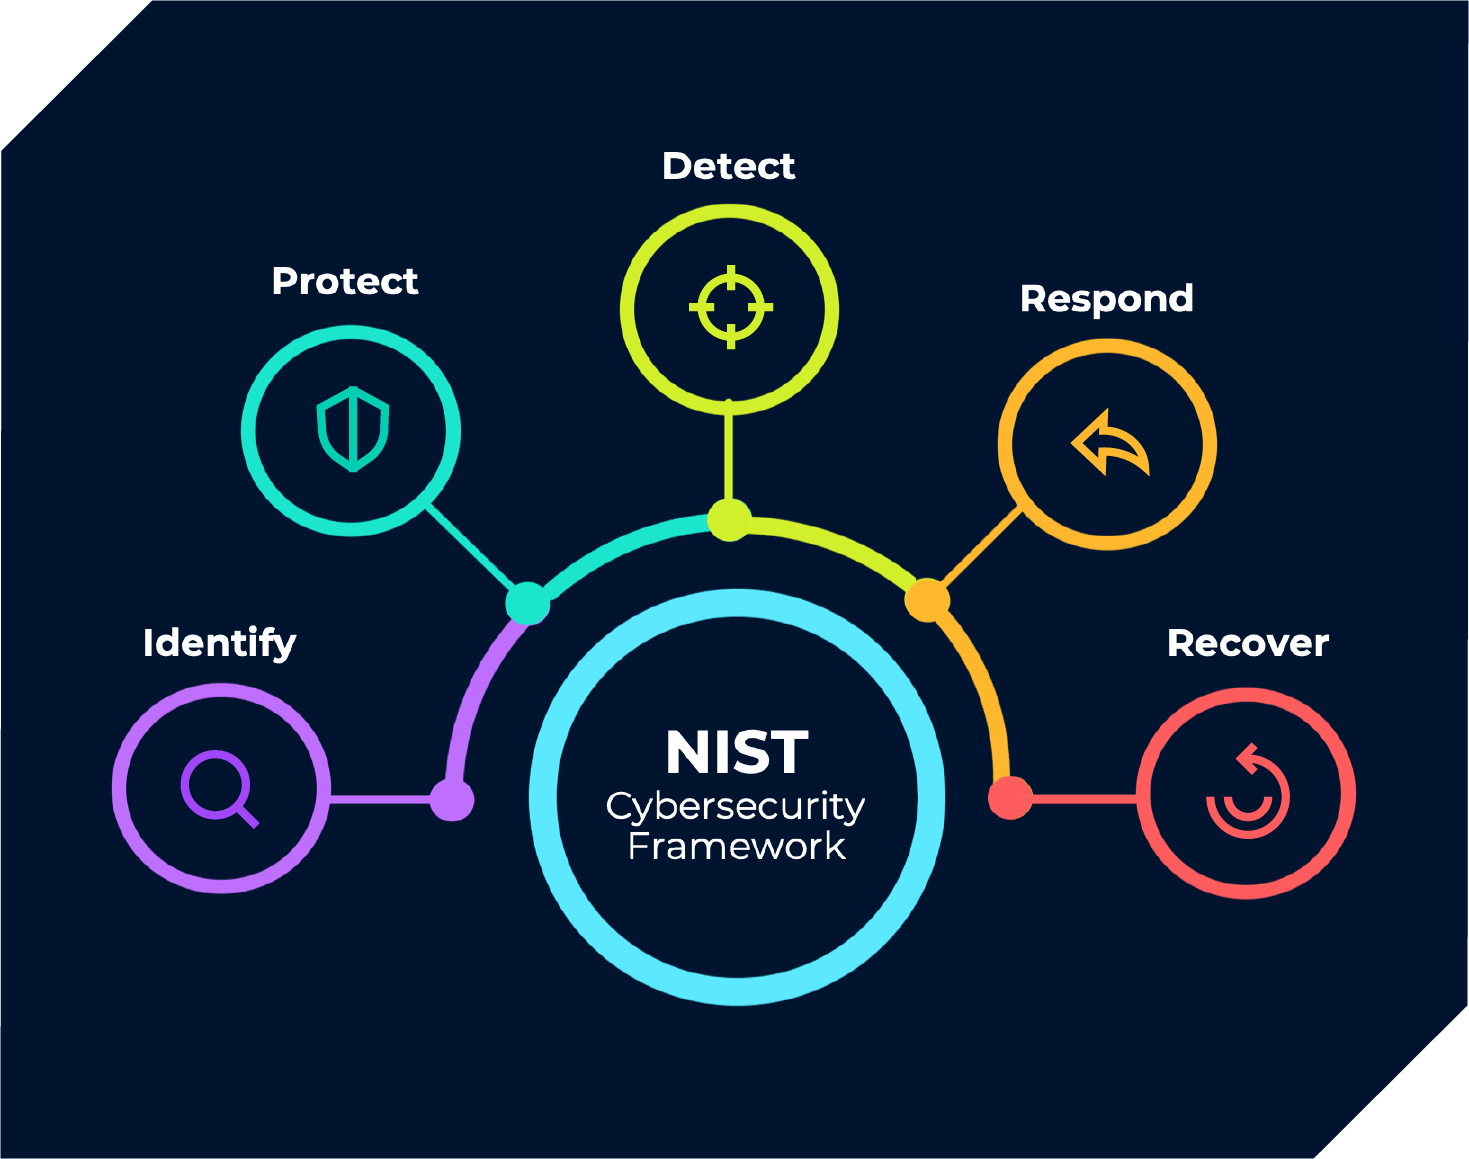
\includegraphics[width=0.8\textwidth]{Figures/qict-working-method.png}
      \caption{\acrshort{nist} working methodology that is followed by \acrshort{qict}}
\end{figure}

\begin{figure}[htbp]
      \centering
      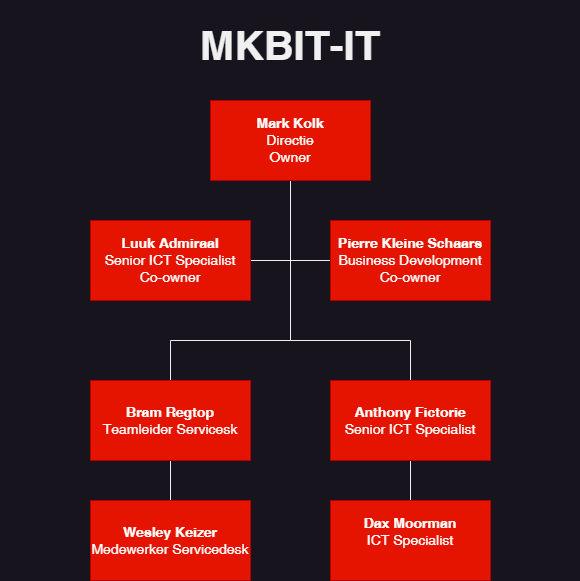
\includegraphics[width=0.8\textwidth]{Figures/Organogram-MKBiT.png}
      \caption{Level of structure of \acrshort{mkb}iT}
\end{figure}

\begin{figure}[htbp]
      \centering
      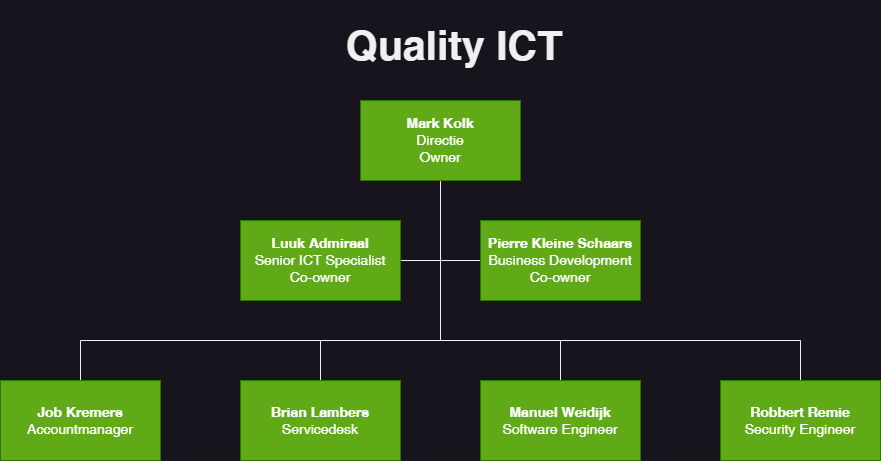
\includegraphics[width=0.8\textwidth]{Figures/OrganizationalDiagram_QICT.png}
      \caption{Flat (hierarchical) structure of \acrshort{qict}}
\end{figure}

\begin{figure}[htbp]
      \centering
      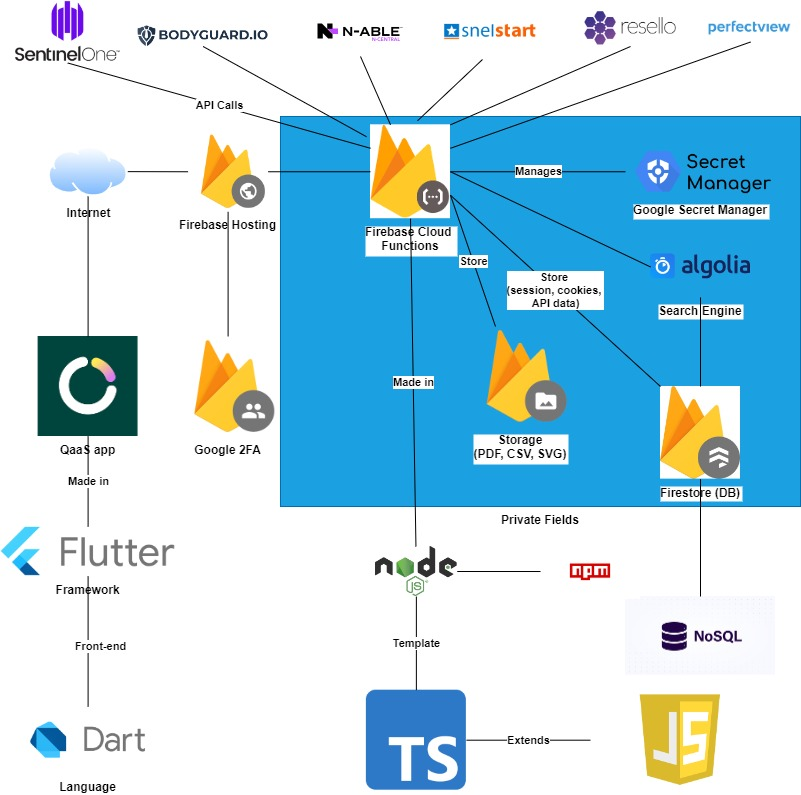
\includegraphics[width=0.8\textwidth]{Figures/QaaS App Infraastructure.jpg}
      \caption{The infrastructure of the QaaS app}
\end{figure}

\begin{multicols}{2}
      \subsubsection{Firebase}
      Firebase is a comprehensive platform for developing and managing web and mobile applications, created by
      Google and is party of \acrshort{gcp}. It was originally an independent company founded by Firebase, Inc.
      in 2011. It was then acquired by Google in 2014. Since then, it has become an integral part of Google's
      broader ecosystem of cloud services (\cite{firebase}). It is a \acrshort{baas} that provides developers with a
      variety of tools and services to help with both back-end infrastructure and front-end capabilities without worrying
      about managing servers or infrastructures. The services offered by Firebase (\textit{\cite{firebaseproducts}}) are
      many, but for this thesis, it will only discuss the ones that are used by the \acrshort{qaas} app. They are listed
      in the following:
      \begin{itemize}
            \item Authentication: is an easy-to-understand authentication services that support various authentication
                  methods like email/password, phone number, with identity providers such as Google, Facebook, Twitter,
                  Apple, GitHub, \acrshort{etc}
                  along with utilizing \acrshort{2fa} authentication factors to enhance security by requiring additional
                  factor, such as an \acrshort{otp} code that is sent to the user's phone or security key.
            \item Database:
                  \begin{itemize}
                        \item Firestore Database: Firestore is a \gls{NoSQL} database that is part of the Firebase
                              platform. It is a flexible, scalable database for mobile, web, and server development. It keeps
                              data in sync across client apps through real-time listeners and offers offline support for mobile
                              and web, so the developers can build responsive apps that work regardless of network latency or
                              Internet connectivity.
                  \end{itemize}
            \item Cloud Functions: often just called Functions in the Firebase console, it allows developers to run
                  back-end code in response to events triggered by Firebase features and \acrshort{https} requests.
                  The code is stored in Google's cloud and runs in a managed environment. It is a serverless framework
                  that allows developers to build and deploy serverless functions that automatically scale up and down
                  based on demand. The available programming languages are Node.js (\acrshort{js} and \acrshort{ts}),
                  Python, Go, Java, and .NET (C\#). Cloud Functions offers 2 product versions: the original version
                  (1st gen), and the 2nd gen which is built on Cloud Run and Eventarc to provide an enhanced feature set.
                  \begin{itemize}
                        \item 1st Generation: Most of the Firebase Cloud Functions that are used in the \acrshort{qaas} app
                              is in this version. The company wishes to migrate all the functions to the 2nd generation in
                              the future.
                        \item 2nd Generation: The company wishes that the author's graduation project will utilize the 2nd
                              generation of Cloud Functions. Features in the 2nd generation including:
                              \begin{itemize}
                                    \item Longer request processing times
                                    \item Larger instance sizes
                                    \item Traffic management
                                    \item Eventarc integration
                                    \item Broader CloudEvents support
                              \end{itemize}
                  \end{itemize}
                  Cloud functions are the main back-end infrastructure of the \acrshort{qaas} app. It is used to connect
                  and make \acrshort{http} calls to all the internal \acrshort{api}s. There are different types of
                  functions in Firebase Cloud Functions, and they will be discussed later.
      \end{itemize}
\end{multicols}

\begin{figure}[htbp]
      \centering
      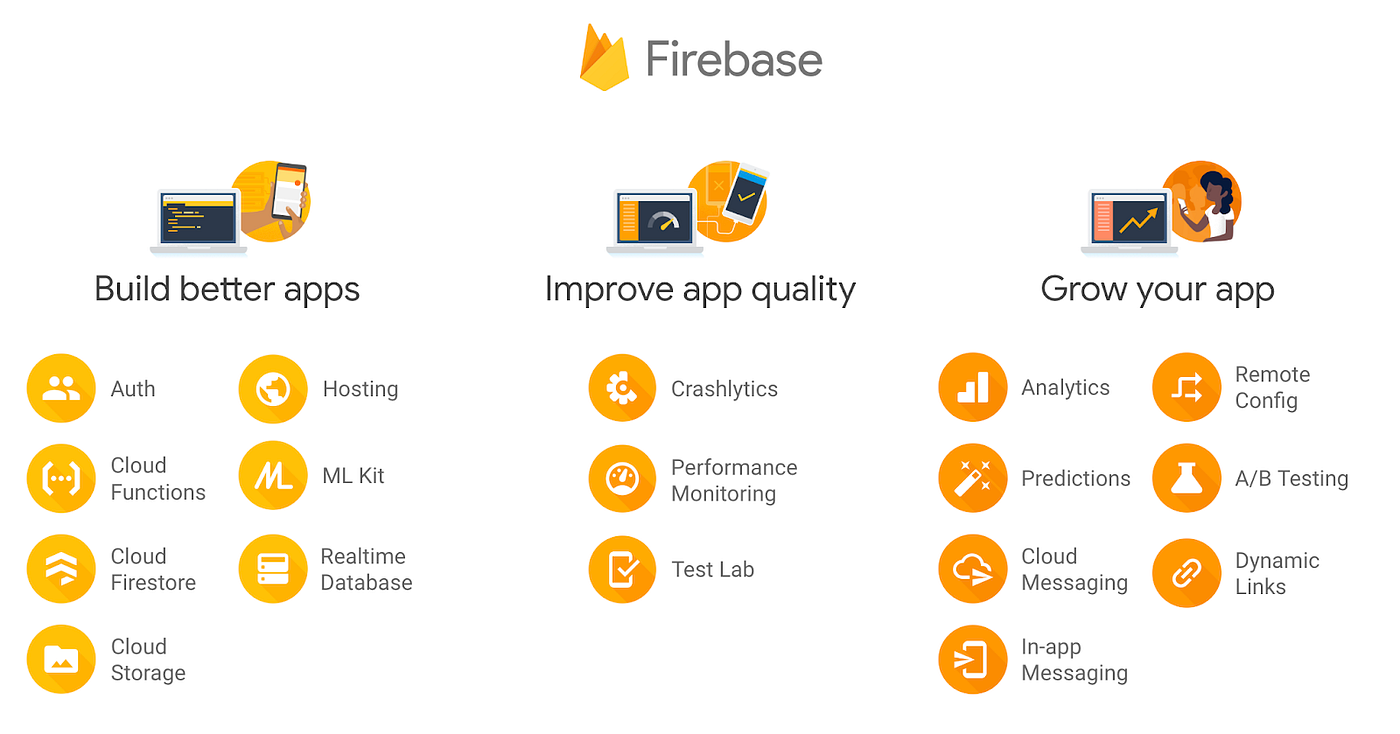
\includegraphics[width=0.8\textwidth]{Figures/Firebase.png}
      \caption{All of the products offered by Firebase (\textit{\cite{firebasePic}})}
\end{figure}

\begin{longtable}{|p{5cm}|p{5.5cm}|p{5.5cm}|}
      \hline
      \rowcolor{blue!20}
      Feature         & 1st Gen                                                     & 2nd Gen                                                       \\
      \endfirsthead
      \hline
      Image registry  & Container Registry or Artifact Registry                     & Artifact Registry only                                        \\
      \hline
      Request timeout & Up to 9 minutes                                             & \begin{itemize}
                                                                                            \item Up to 60 minutes for \acrshort{http}-triggered functions
                                                                                            \item Up to 9 minutes for event-triggered functions
                                                                                      \end{itemize} \\
      \hline
      Instance Size   & Up to 8\acrshort{gb} \acrshort{ram} with 2 v\acrshort{vcpu} & Up to 16\acrshort{gb} \acrshort{ram} with 4 \acrshort{vcpu}   \\
      \hline
      Concurrency     & 1 concurrent request per functions instance                 & Up to 1000 concurrent requests per function instance          \\
      \hline
      \caption{Comparison between the 1st and 2nd Generation of Cloud Functions}
      \label{tab:restvsoap}
\end{longtable}

\begin{figure}[htbp]
      \centering
      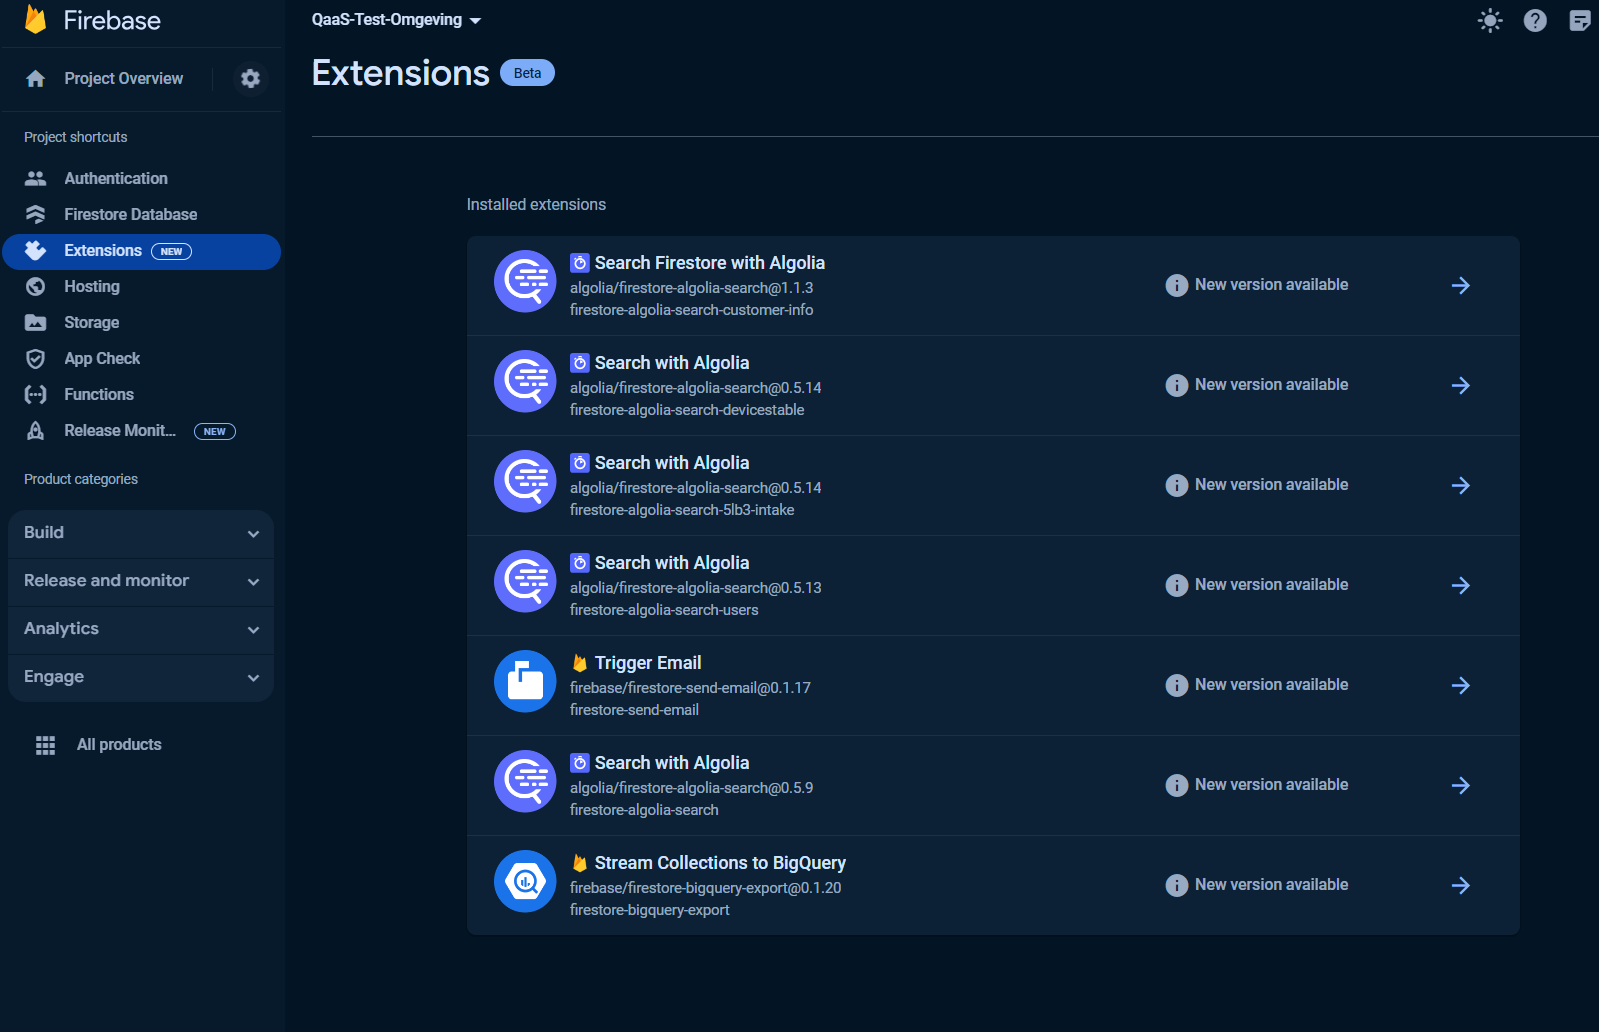
\includegraphics[width=0.8\textwidth]{Figures/Firebase/Extensions.png}
      \caption{All the extensions that are used in the \acrshort{qaas} app, mostly about Algolia}
\end{figure}

\begin{figure}[htbp]
      \centering
      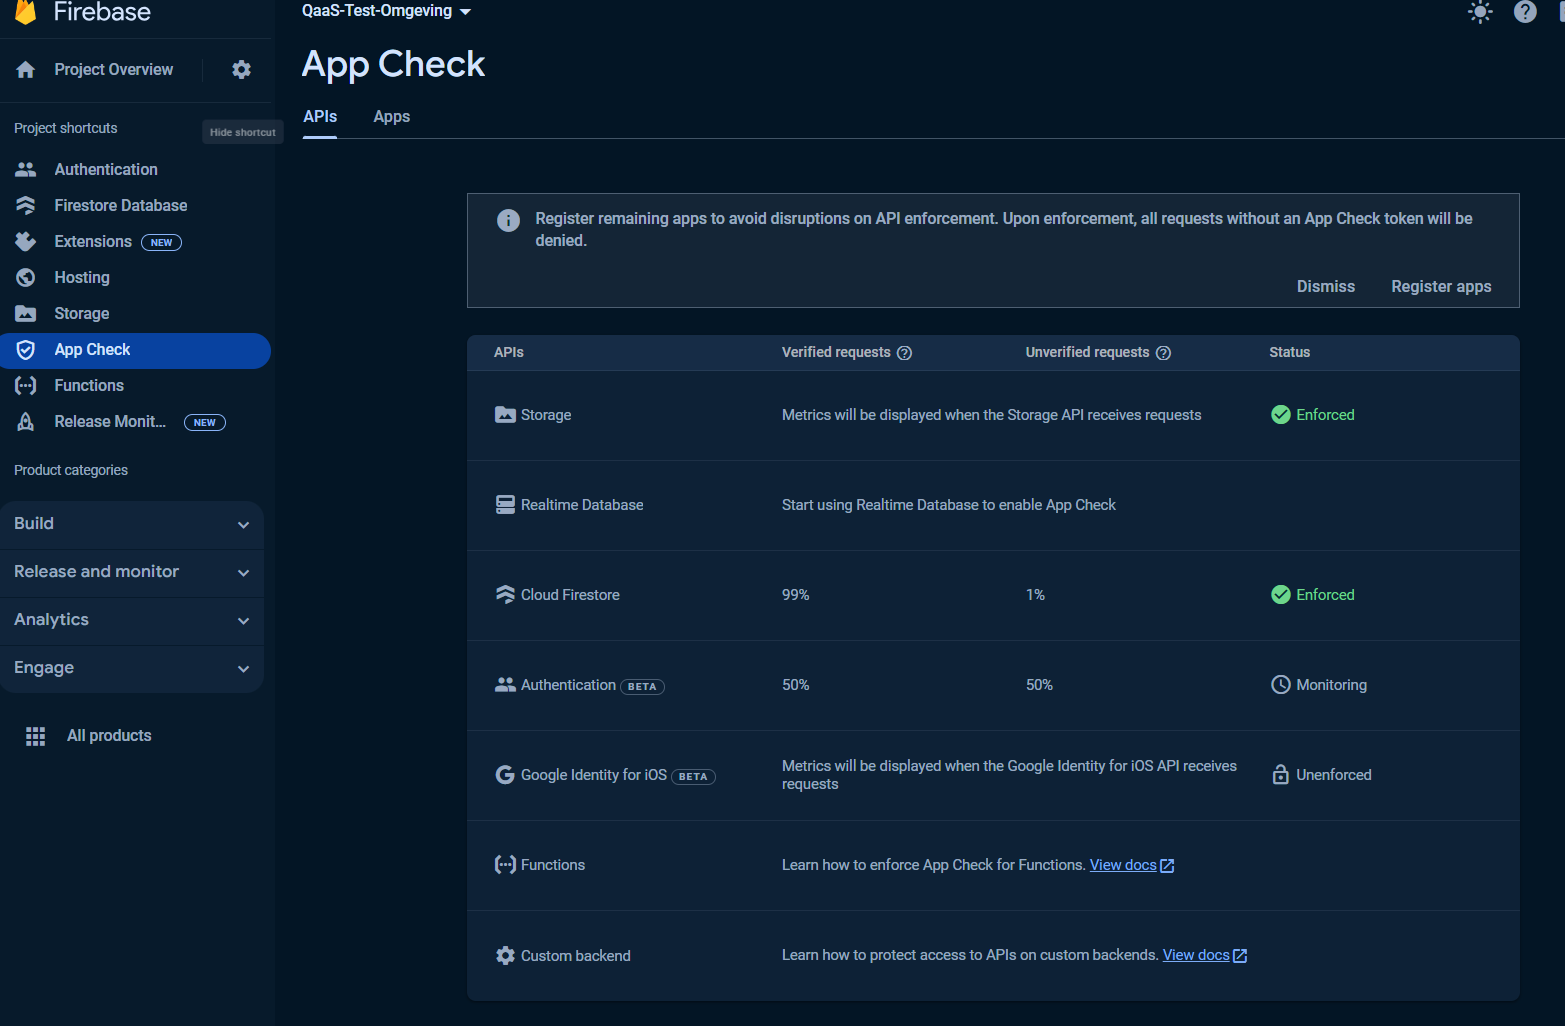
\includegraphics[width=0.8\textwidth]{Figures/Firebase/App Check.png}
      \caption{The App Check feature in the \acrshort{qaas} app}
\end{figure}

\begin{figure}[htbp]
      \centering
      
\includegraphics[width=0.8\textwidth]{Figures/Firebase/Functions/CronJobs.png}
      \caption{The function in the \acrshort{qaas} app that is scheduled to run every 7 days to keep the \acrshort{api} data up-to-date
            (\textit{\cite{cronJobQaaSAppFunction}})}
\end{figure}

\begin{lstlisting}[language=JavaScript, caption=Example of onCall function with authentication check]
      const region = "europe-west1";

      const getData = functions.https.onCall({ region: region }, async (request: CallableRequest<any>) => {
            try {
                  // Checking that the user is authenticated.
                  if (!context.auth) {
                        // Throwing an HttpsError so that the client gets the error details.
                        throw new functions.https.HttpsError('failed-precondition', 'The function must be called while authenticated.');
                  }
            }
            catch (ex: unknown) {
                  if (error instanceof Error) {
                        // Error object, log message and stack if available
                        console.error(`[${context}] An error occurred: ${error.message} \n Stack: ${error.stack}`);
                  } else {
                        // Non-Error object, log with a generic message.
                        console.error(`[${context}] An unknown error occurred:`, error);
                  }
                  throw new functions.https.HttpsError("unknown", "Failed to retrieve agents", ex);
            }
      });
              
      export = getData;
\end{lstlisting}

\begin{multicols}{2}
      \begin{itemize}
            \item Hosting: a service that allows developers to host static websites, dynamic web apps, mobile apps, and
                  microservices on Firebase's infrastructure. The \acrshort{qaas} app is currently hosted on Firebase
                  Hosting.
            \item Cloud Storage: offers secure, scalable, and reliable file storage and sharing for Firebase apps.
                  It is designed to help developers quickly and easily store and serve user-generated content, such as
                  photos or videos. It is used by the \acrshort{qaas} app to store and serve user-generated content, such as
                  profile pictures, documents, and other files.
            \item Extensions: it consists pre-built, open-source software packages that extend the functionality of a Firebase
                  project (\textit{\cite{firebaseExtension}}). They are designed to automate common development tasks, such as
                  sending notifications, integrating with third-party services, and performing back-end operations, without
                  requiring users to write custom code. The \acrshort{qaas} app uses the Extension mainly for Algolia.
            \item App Check: it is a security feature that, on top of Firebase \acrshort{2fa} Authentication, that helps protect
                  the project from abuse, such as billing fraud or phishing, by ensuring that only the app that is registered
                  can have access to the Firebase project's resources (\textit{\cite{appCheckFirebase}}). In the case of the
                  \acrshort{qaas} app, it uses it \gls{reCAPTCHA} to ensure extra protection in the \acrshort{mfa}.
      \end{itemize}

      \textbf{Different Types of Cloud Functions in Firebase}

      Firebase has a lot of different types of Cloud Functions that developers can use. Just like the previous Firebase product
      explanation, this thesis will only focus on the following types of Cloud Functions that are used in the \acrshort{qaas} app:

      \textbf{HTTP Triggers}: these are functions that are triggered by \acrshort{http} requests. They are used as \acrshort{api}
      endpoints of the \acrshort{qaas} app, allowing server-side logic execution in response to \acrshort{http} requests from
      client-side applications or external services. The requests are GET, POST, PUT, DELETE, and PATCH, and they are used to
      creating, reading, updating, and deleting data in either the Firestore \acrshort{db} or the correlated \acrshort{api}
      environment itself.

      \begin{itemize}
            \item onRequest:
            \item onCall: is a little different from onRequest. Instead of using Request and Response, it uses data and context.
                  In version 2.0, it only accepts request as \texttt{CallableRequest<any>} that can get any headers and body
                  of the request sent by user. It is used to create Callable Functions, and they are designed to be called directly
                  from client applications, such as mobile or web apps. They automatically handle authentication and data serialization,
                  making it easier to secure call backend code from client applications, and this is what the \acrshort{qaas} app
                  primarily uses for calling its internal \acrshort{api}s as it ensures that the client is authenticated and authorized
                  to make the call. Callable functionsa are triggered by an \acrshort{http} request but are specifically designed to be
                  called from Firebase client \acrshort{sdk}s.

      \end{itemize}

      \textbf{Pub/Sub Triggers}

      \textbf{Cloud Firestore}

      \textbf{Schedule functions}: this is a Firebase's own term for \gls{cronJob} (\textit{\cite{scheduleFunction}}).

      \textbf{Algolia}

      Algolia is used for search functionality. It is a search-as-a-service platform that enables developers to
      integrate and build fast, relevant search functionality into their applications and websites
      (\textit{\cite{algolia}}). It provides a range of features and capabilities for building and managing search
      functionality, including full-text search, typo tolerance, and relevance tuning, as well as analytics and
      monitoring tools to help developers understand how users are interacting with their search functionality in
      real-time.

      The reason as to why \acrshort{qict} uses Algolia is that the nature of Firebase search engine is quite often
      proven to be inaccurate and slow.

      \textbf{Google Secret Manager}

      It is a fully managed service provided by \acrshort{gcp} that allows developers and organization to securely store,
      access, and manage sensitive information such as API keys, passwords, certificates, \acrshort{oauth} credentials,
      \acrshort{db} credentials and other credentials used in throughout the lifecycle of their applications
      (\textit{\cite{googlesecretmanager}}). It is not part of Firebase, and it helps the \acrshort{qaas} app to centralize and
      secure its secrets in scalable and easily manageable way. Key-features of Secret Manager include:

      \begin{itemize}
            \item Secure Storage: it encrypts the secret values using \acrshort{cmek}, ensuring the sensitive data is protected
                  both at rest and in transit.
            \item Audit Logs: it provides and manages audit logs that record all access and modification of activities, helping
                  developers meet compliance, better accountability and regulatory requirements.
            \item Versioning and Automatic Rotation: it supports versioning of secrets, allowing developers to store multiple versions
                  of the same secret. This means that the developers get to keep multiple versions of secrets and easily revert or roll
                  back to a previous version if needed, which will help in auditing and tracking changes to secrets over time. This feature
                  enables automatic seamless rotation of secrets at regular intervals without  disrupting the applications, which improves
                  the security part of the application by ensuring that secrets are regularly updated without manual intervention.
            \item Access Control: it provides fine-grained access control using Google \acrshort{iam}, allowing developers to specify
                  who can access and manage the stored secrets and what they can do with them.
            \item Centralized Management: it stores and manages all secrets in one place, simplifying access and control.
      \end{itemize}

      Google Secret Manager comes from \acrshort{gcp}, and \acrshort{gcp} and Firebase are a separate cloud solutions. But, because
      both are part of Google, Firebase Cloud Functions can typically access \acrshort{gcp} Secret Manager by editing that specific function
      that the developer wanted to grant access to.
\end{multicols}

\begin{multicols}{2}
      \subsubsection{Different Types of API By Audience}
      To understand better about the 5 internal \acrshort{api}s that are used by the \acrshort{qaas} app, including SentinelOne,
      it is important to understand the different types of \acrshort{api}s by its audience and protocol. There are 3 main types of
      \acrshort{api}s by audience, they are:

      \textbf{Public API}: also called external or Open \acrshort{api}, and as the name suggests it is available
      to everyone. They are open to the public to use and integrate with their applications. Developers can quickly
      implement them using little to no authorization, with few require sign-up and generation of the \acrshort{api} Keys
      to access them. This can make them to not be the best regarding security - just because "public" means expanded
      visibility - but sharing data with them is easier.

      Examples of a public \acrshort{api} are OpenWeatherMap, Google Maps navigation, Facebook and the Twitter \acrshort{api},
      which the latter allows  developers to access Twitter's functionality and data.

      \textbf{Internal API}: also called Private \acrshort{api}, and is used within a private organization to make internal
      apps "talk" to each other. To interact with the data, a developer needs to be actively granted permission to access it,
      because the data and functionality available through the \acrshort{api} are proprietary to the company. They are often
      set up with extensive logging and load-balancing capabilities because they must have greater fault tolerance and
      security than public \acrshort{api}s. They also do not follow the Open\acrshort{api} standard as consistently
      as public \acrshort{api}s, since their producers and consumers typically work together closely, data formats
      can be negotiated based on specific use cases. As they are built by specifically the company; it will only have
      \acrshort{api} protocol types that the organization wants to support. All the \acrshort{api}s managed by the
      \acrshort{qaas} app fall into this category. This solution tend to be very secure, as they are entirely internal.

      \textbf{Partner API}: also called Shared \acrshort{api}, this \acrshort{api} is made considering the scalability
      while developing the business, which will share a few \acrshort{api}s across a few other licensed organizations,
      enabling service offerings across business (\acrshort{b2b}). This \acrshort{api} is shared only with the intended
      users; others might not have access to them because they are not shared publicly, thus making it exists somewhere
      between public and private \acrshort{api}s. They often function to share data between two companies or organizations
      for a specific business purpose, while still ensuring strict privacy protection.

      These \acrshort{api}s indeed require authorization to access them (like having a PayPal account or an \acrshort{api}
      key). All the clients who are part of the business can access and integrate using those \acrshort{api}s. Few
      \acrshort{api}s will only provide read access, and few will provide read/write access via shared \acrshort{api}s.
      This depends on the business process model.

      For example, travel booking \acrshort{api}s are shared with travel agencies to increase their visibility and
      booking. Websites like Expedia, Make My Trip, and Trivago are excellent examples of this kind of \acrshort{api}.

      \subsubsection{Different Types of API Protocols}\label{chap:typesofapis}
      \textbf{\acrshort{soap} \acrshort{api}s}: are strictly based on \acrshort{xml} for the message structure and
      \acrshort{http} for the protocols. \acrshort{soap} itself is a protocol and sending a \acrshort{soap}
      request is like using an envelope to send a message. \acrshort{soap} \acrshort{api}s consume extra
      overhead and more bandwidth, and require more work on both the client and server ends. Like envelopes,
      \acrshort{soap} encloses more stringent security compared to \acrshort{rest}. \acrshort{xml}-encoded
      \acrshort{soap} messages use the format defined below:
      \begin{itemize}
            \item \textbf{Envelope}: the root element of the message, which encapsulates the entire
                  \acrshort{soap} message. It 'envelopes' the message by placing tags at the start and the end.
            \item \textbf{Header (optional)}: defines specific additional message requirements, such as authentication.
            \item \textbf{Body}: the request of response is included here.
            \item \textbf{Fault (optional)}: information about errors that might arise during the execution of the
                  \acrshort{api} call or response is highlighted here, along with information on how one can address
                  these errors.
      \end{itemize}
\end{multicols}

\begin{lstlisting}[language=XML, caption=Example of a SOAP request, label=lst:soaprequest]
      <SOAP-ENV:Envelope xmlns:SOAP-ENV="http://schemas.xmlsoap.org/soap/envelope/" xmlns:example="http://example.com">
            <SOAP-ENV:Header/>
            <SOAP-ENV:Body>
                  <example:GetUser>
                        <example:UserID>123</example:UserID>
                  </example:GetUser>
            </SOAP-ENV:Body>
      </SOAP-ENV:Envelope>
\end{lstlisting}

\begin{multicols}{2}
      \textbf{REST API}: if \acrshort{soap} is like an envelope, \gls{REST} is like a  more lightweight postcard.
      \acrshort{rest} \acrshort{api}s are considered the gold standard for scalability and are highly compatible with
      microservice architecture. It is the often used protocol in the context of building \acrshort{api}s for web-based
      applications. \acrshort{rest} itself is not a protocol, but an architectural style for designing networked
      applications, defining a set of constraints and principles that define how web services should be structured
      and interact with each other.

      \acrshort{api}s that follow \acrshort{rest} principles are called \acrshort{rest}ful \acrshort{api}s. The
      are \acrshort{rest}ful as long as they comply with the 6 guiding constraints of a \acrshort{rest}ful system
      (\cite{restguidingprinciples}):
      \begin{itemize}
            \item \textbf{Client-server architecture}: the architecture is composed of clients, servers, and
                  resources, and it handles requests through \acrshort{http}.
            \item \textbf{Statelessness}: no client is stored on the server between requests. The server should
                  process and complete each request independently. Information about the session state is, instead,
                  held with the client. The clients can do this via query parameters, headers, \acrshort{uri}s,
                  request body, \acrshort{etc}
            \item \textbf{Cacheable}: simply, the clients should be able to determine whether this response is cacheable
                  from their side, and if so, for how long. If a response is cacheable, the client has the right to return the
                  data from its cache for an equivalent request and specified period, without sending another request to the
                  server. A well managed caching mechanism can eliminate the need for some client-server interactions
            \item \textbf{Layered system}: client-server interactions can be mediated by additional layers. These
                  layers could offer additional features like load balancing, shared caches, or security.
            \item \textbf{Uniform interface}: this is the core to design \acrshort{rest}ful \acrshort{api}s.
                  There should be a uniform and standard way of interacting with a given server for all client
                  types. The uniform interface helps to simplify the overall architecture of the system. This includes
                  4 facets:
                  \begin{itemize}
                        \item Resource identification in request: resources are uniquely identified in requests and are separate
                              from the representations that are returned to the client using \acrshort{uri}.
                        \item Resource manipulation through representations: clients receive files of a uniform that represent resources.
                              These representations must have enough information to allow modification or deletion of the resource's
                              state in the server, as long as they have the required permissions.
                        \item Self-descriptive messages: each message returned to a client contains enough information to describe
                              how the client should process the information further, such as additional actions that can be
                              performed on the resource.
                        \item Hypermedia as the engine of application state: after accessing a resource, the \acrshort{rest} client
                              should be able to discover through hyperlinks all other actions that are currently available.
                  \end{itemize}
            \item \textbf{Code on demand (optional)}: servers can extend the functionality of a client by transferring
                  executable code.
      \end{itemize}
      \acrshort{rest} \acrshort{api}s are high-performing (especially over \acrshort{http}2), time-tested, and support
      many data formats. They also decouple the client and server, making sure of independent evolution. However,
      building a true \acrshort{rest} \acrshort{api} is difficult because it requires a disciplined adherence to the
      Uniform Interface constraint (\cite{restapiuniforminterface}). Some organizations trade off the long-term benefits
      of a truly \acrshort{rest} \acrshort{api} for other \acrshort{http} \acrshort{api} protocols that have similar
      benefits but adhere to \acrshort{rest} constraints more liberally. \acrshort{rest} requests typically include these
      key components:
      \begin{itemize}
            \item \textbf{Endpoint}: the uniform resource identifier that locates the resource on the internet is
                  part of this component. \acrshort{url}s are the most common type of \acrshort{uri}.
            \item \textbf{HTTP Method}: this component outlines the four basic processes that a resource can be subjected
                  to: POST (create a resource), GET (retrieve a resource), PUT (update a resource), and DELETE
                  (remove a resource).
            \item \textbf{Headers}: data related to the server and the client are stored in this component. Like in
                  \acrshort{soap}, one can also use \acrshort{rest} headers to store authentication measures such as
                  \acrshort{api} keys, server \acrshort{ip} addresses, and the response format.
            \item \textbf{Body}: this component contains additional information for the server, such as data that needs to
                  be added or replaced.
      \end{itemize}
\end{multicols}
\begin{lstlisting}[language=JavaScript, caption=Different HTTP methods in REST]
            GET /users <@\textnormal{Retrieve list of all users}@>
            GET /users/{id} <@\textnormal{Retrieve details a specific user by their ID}@>
            POST /users <@\textnormal{Create a new user}@>
            PUT /users/{id} <@\textnormal{Update a specific user by their ID}@>
            DELETE /users/{id} <@\textnormal{Delete a specific user by their ID}@>
\end{lstlisting}
\begin{lstlisting}[language=JavaScript, caption=REST's Example Request]
            GET https://api.example.com/users/123
\end{lstlisting}
\begin{lstlisting}[language=JavaScript, caption=Example of REST request in JavaScript]
      const apiUrl = 'https://api.example.com/users/123';

      // Define the request parameters
      const requestOptions = {
            method: 'GET', // HTTP method (GET, POST, PUT, DELETE, PATCH, etc.)
            headers: {
                  'Content-Type': 'application/json', // Set the content type of the request
            }
      };

      // Make the API request
      fetch(apiUrl, requestOptions)
            .then(response => response.json())
            .then(data => console.log(data)) // Process the response data
            .catch(error => console.log('error', error)); // Handle any errors that occurred during the request
\end{lstlisting}
\begin{multicols}{2}
      All three of the \acrshort{rest}, \acrshort{soap}, and Graph\acrshort{ql} use the \acrshort{http} protocol for
      communication therefore falls into \acrshort{http} \acrshort{api}s category. They are the commonly used for web
      services  and allow applications to interact with each other over the internet. \acrshort{http} is superbly
      suited for applications following a request-response paradigm.

      \subsubsection{Modules and Templates of the QaaS App}

      The \acrshort{qaas} has several templates and modules that are used to build the app. The templates can be
      interpreted as level of access to the app, showing what permission a user has to the app. There are 3 different
      templates based on 3 different users:

      \begin{itemize}
            \item \textbf{Clients}: this template is used by the general users of the app. They have limited access to
                  the app's features and functionalities, such as viewing and updating their profile and accessing the app's
                  resources. They can only see the data relevant to their own account and cannot access or modify data
                  belonging to other client from different company.  The Client template is designed for users who have the
                  lowest level of access and control over the app.
            \item \textbf{Helpdesk}: this template is used within the Helpdesk department of \acrshort{qict}. They have more
                  access to the viewing of app functionality than the Clients.
            \item \textbf{IT Admin}: the \acrshort{it} admin have almost the same level of access as the Helpdesk. The only
                  difference is that they have the ability to create, edit, and delete users, manage user permissions, and
                  configure the app settings. They can also grant and revoke access to a user and to the app's features and
                  functionalities, which are called Modules. The admin template is designed for users who have the highest level
                  of access and control over the app, which is to the developers.
      \end{itemize}

      Modules are

      \section{Research Sub-Question \#2}
      \subsection{SentinelOne} % vs CrowdStrike with Carbanak and FIN7 methodology, Huntresss, datto rmm
      To answer this research sub-question, a general understanding of what SentinelOne is needed to know what
      methods should be utilized to integrate it with the \acrshort{qaas} app.

      SentinelOne is a cybersecurity platform that provides endpoint protection, detection, and response capabilities to
      help organizations defend against advanced cyber threats. It leverages \acrlong{ai} and machine learning to analyze
      and respond to security threats in real-time, providing organizations with comprehensive protection against malware,
      ransomware, and other cyber threats. It also provides visibility into clients' \acrshort{it} systems and infrastructure,
      enabling organizations to gain insights into potential security risks and vulnerabilities and take proactive measures
      to address them.

      Some terminology that the readers need to be familiar with before diving deeper into SentinelOne:

      \textbf{Endpoint}

      Endpoint can be defined as any remote computing devices that receives incoming communications and sends outgoing messages
      to the network it is connected to. Examples of endpoints include desktops, laptops, smartphones, tablets, servers, workstations,
      and other \acrshort{iot} devices that is connected to a network. They are the first-line of defence for the Blue Team today.

      Examples of endpoints are:
      \begin{itemize}
            \item Computer (workstations, desktops)
            \item Laptop
            \item Server
            \item Mobile devices
      \end{itemize}

      \textbf{EPP}

      \acrshort{epp} is an upgrade from legacy \acrshort{av}/anti-malware. \acrshort{epp} consists of solutions that work together to detect
      and block security threats at the endpoint device level.

      Important note that \acrshort{epp} is not to be confused with \acrshort{edr}. \acrshort{epp} is a separate service from \acrshort{edr},
      in which in \acrshort{edr} platforms they often include \acrshort{epp} but not vice versa.

      \textbf{EDR}

      \acrshort{edr} \acrshort{aka} \acrshort{etdr}, is a group of integrated endpoint security solutions that combine data collection,
      data analysis, forensics, and \gls{threathunting} with the end-goal of identifying and stopping any potential security breaches in due
      time. \acrshort{edr} solutions are able to recognize any suspicious patterns that can be investigated later on, as they have been
      purposefully created to detect and respond in an active manner to advance malware, ransomware, and other cyber threats (the Response
      \acrshort{edr}). \acrshort{edr}, as the name suggest, were developed specifically for endpoints, and not networks (\ref{sec:ndr}), thus
      operate only on endpoint level.

      The number one thing that sets apart \acrshort{edr} from legacy (traditional) \acrshort{av} is that traditional \acrshort{av} relies on
      signature-based detection, usually having a defined set of list in their \acrshort{db}, where known malware signatures are compared
      against files or processes to identify threats. \acrshort{edr} on the other hand, uses a combination of signature-based detection, such
      as behavioural analysis, machine learning, and anomaly detection to identify and respond both known and unknown threats. \acrshort{edr}
      solutions focus on detecting malicious activities at the endpoint level, including file modifications, process execution, and network
      connections, focusing on malicious behaviour compared to only concerning with malicious software like what traditional \acrshort{av} does.

      \textbf{MDR}

      \acrshort{mdr} is what manage the \acrshort{edr} technology.

      \textbf{NDR} \label{sec:ndr}
      \acrshort{ndr} products are designed to provide a complete visibility into the network, real-time detection of threats, and guided
      investigation to accelerate and automate responses (\textit{\cite{sentinelOneNDR}}). \acrshort{ndr} takes a feed of raw network traffic
      from a \gls{networkTap}, port mirror, or virtual traffic mirroring in \acrshort{aws} and Azure. By analyzing this traffic in real-time,
      \acrshort{ndr} finally discovers and classify every device communicating on the network. It identifies device roles, such as \acrshort{dns},
      web server, medical device, \acrshort{etc} and maps peer groups among those devices.

      \textbf{SIEM}

      is a software system that collects, aggregates, normalizes security data from a variety of sources within an IT infrastructure, and
      analyzes it according to pre-set rules, present it in human-readable format and therefore giving a comprehensive picture of the company's
      information security (\cite{siemGartner}). \acrshort{siem} tools evolved from the log management discipline and combine \acrshort{sim} and
      \acrshort{sem} technologies. A \acrshort{siem} tool uses \acrshort{ai} to automate several manual procedures related to threat
      detection and incident response. Furthermore, it assists enterprise security teams in spotting anomalies in user behavior.

      \begin{itemize}
            \item Input: logs, threat intel, vulnerability feeds, \acrshort{ndr}, firewall, \acrshort{ips}, \acrshort{ids}, and \acrshort{edr}
                  data
            \item Output: high-fidelity alerts prioritized by severity
            \item Infused with: \acrshort{ai}, \acrshort{ml}, and analytics
      \end{itemize}

      \textbf{SOAR}

      \acrshort{soar} solutions focus on automating incident response processes and triage capabilities. The key word here is
      "orchestration" and "automation". In an ideal world, everything.
      The main goal is to oversee security without human help as much as possible, boosting productivity and shortening the response time.
      It might use \acrshort{ai} and \acrshort{ml} to assess security events and automate incident response procedures. These solutions
      can be standalone product, or it can be added to \acrshort{siem} solutions since \acrshort{soar} does not excel in event analysis.

      \textbf{XDR}

      is a security solution that gathers and analyzes data from multiple sources like endpoints, networks, cloud, emails, app,
      \acrshort{etc} It offers great visibility into a company's \acrshort{it} infrastructure, helping the security employees to detect
      more threats, respond efficiently, and deal with fewer false positive alerts \cite{xdrIDC}.

      This solution integrates several tools combining all the gathered data into a single platform to visualize the information. It might
      incorporate automated processes (even complex ones), \acrshort{ml}, and advanced analytics to enable quicker and more effective
      incident response. It can even deal with hidden and advanced malware.

      \textbf{MXDR}

      Some people may still call it \acrshort{mdr}, managed \acrshort{soc}, or managed security.

      \textbf{SOC}

      \acrshort{soc} is the organizational context itself. It is a centralized facility or team within an organization that houses a
      security team responsible for monitoring and analyzing another organization's (client) security position on an ongoing basis. They
      can be seen as the safety team for client organizations. Please note that SentinelOne company itself is not a \acrshort{soc}, as it
      is just a cybersecurity company that offers endpoint security solutions.

\end{multicols}

\begin{figure}[htbp]
      \centering
      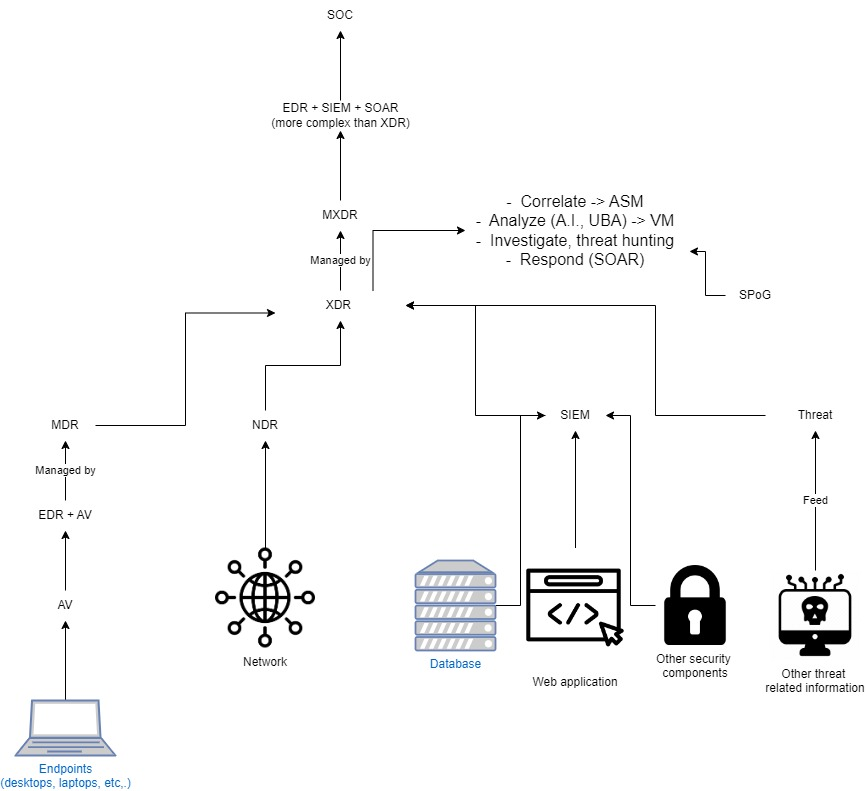
\includegraphics[width=0.8\textwidth]{Figures/XDR.jpg}
      \caption{How all terms related to various technologies in cybersecurity connected to each other}
      \label{fig:xdr}
\end{figure}

\begin{multicols}{2}
      \textit{Please note that as mentioned before, \acrshort{siem} can also take data from an \acrshort{edr} and \acrshort{ndr} but for
            the sake of simplicity, the diagram puts them as a separate pier systems}. In terms of SentinelOne, it has all the features that
      are mentioned in the diagram, except for \acrshort{soc}, as was mentioned before.

      \textbf{Console}

      \textbf{Global}

      The Global tab refers to the environment of the highest level of advisors. It consists of organizations that have access to global level
      that propagate down to the tenant level, which means they can put policies, scripts, and other configurations that will be applied to all
      console and all of their customers.

      \textbf{Tenant}

      \textbf{Mentees}

      \textbf{Site}

      Site is just a name

      \textbf{Group}

      Group refers to logical grouping of devices within SentinelOne \acrshort{mgmt} Console. Groups can be created and deleted by the
      admin user, and

      \textbf{Agents}

      An Agent is a software program, part of SentinelOne product, that is deployed to each endpoint, including desktop, laptop,
      server or virtual environment, and runs autonomously on each device, without reliance on Internet connection, enabling data
      gathering, detection, and response to actions. Agents can be interpreted as an \acrshort{av}, collecting relevant security
      telemetry such as:
      \begin{itemize}
            \item Running processes
            \item Connected servers
            \item Open files
      \end{itemize}
      This information can be useful to detect the presence of a threat or to use in forensic analysis and investigation after
      an attack has occurred (Recovery).

      \textbf{Ranger}

      Ranger is an add-on SentinelOne product that provides a way of detecting other devices (computers and
      \acrshort{iot} devices) that are on the client's computer network. If a malicious attacker comes in and plugs his device
      into the network, all the other SentinelOne agents are going to read the network traffic, determine and classify whether
      that is a new device or a rogue device. As long as a device has Ranger on that network subnet, SentinelOne can gather and
      detect technical information regarding the device.

      \begin{itemize}
            \item Not reviewed
            \item Not trusted
            \item Under analysis
            \item Allowed
      \end{itemize}

      Ranger is designed to detect and take out malicious actors that are in the local subnet, as they can a lot of information about the
      devices (\textit{see \acrshort{arp} Poisoning \cite{arpSpoofing} and man-in-the-middle-attack \cite{man-in-the-middleAttack}}).
      In the real-business scenario, a lot of the times, a company has a very secure perimeter firewall
      (\textit{the big outer castle wall in castle-and-moat network security model \cite{castleMoatWallNetwork}}), but the inside network
      are wide open (unless they are doing logical separations of their local network, such as using \acrshort{vlan}) for attacks inside
      the network.

      Unfortunately for this project scope, Ranger \acrshort{api} calls are off limit, as the company is still..., therefore displaying all
      the Ranger ability to scan and the \acrshort{api} call of the author's account.

      \textbf{Sentinels}

      Sentinels refer to a term that describes SentinelOne ability to deploy and manage security agents on endpoints within an
      organization, not part of SentinelOne product, like Ranger. This is part of the SentinelOne \acrshort{edr} capabilities,
      where the user admin can deploy the agents on the endpoints, and manage them from the SentinelOne console. The admin can
      also create policies, scripts, and other configurations that will be applied to all the agents in the network.

      \textbf{Visibility}

      Unfortunately, \acrshort{qict} does not have Visibility turned on its tenant, thus this feature is also off limit for this project
      scope. But in general, Visibility allows users to do deep querying to be able to identify different things, such as attributes of
      a machine. It is useful when user is looking for threats or any additional information in Incident Response or \gls{threathunting},
      which in most cases is proactive, Visibility can give the user a lot of power to use queries, and interrogate all the information
      or telemetry that SentinelOne has pulled off from the connected machines.

      \textbf{Incidents}

      Incident is just a name of a page in SentinelOne dashboard that provides a list of cyber-incidents overview that have happened on all
      endpoints detected by Agents in the network connected to SentinelOne by Ranger. The page typically offers an overview of all detected
      security incidents, categorized based on severity levels of types of threats.

      Once a threat is detected, the user can take the following actions in the dashboard, if they have enough privileges
      to do so:
      \begin{itemize}
            \item Kill: stops all processes related to that threat
            \item Quarantine: encrypts and moves the threat and its executables
            \item Remediate: deletes all files and system changes created by the threat
            \item Rollback: restores files and configuration that the threat changed. This step is usually taken when a malware has
                  executed its script and has made changes to the system, \acrshort{eg} a ransomware has encrypted all the files and
                  asked for a ransom. By taking this step, all the three previous steps will also be undertaken as well. This will
                  then reboot the system and restore it to the safe state before the malware has been executed.
      \end{itemize}

      \textbf{Reports}

      The reports in SentinelOne provide users with insights into the security posture and threat landscape across their organization's
      endpoints. The reports offer customizable reporting capabilities, allowing users to generate reports tailored to their specific
      requirements. Users can then choose from a variety of predefined report templates or create custom reports based on their unique
      needs.

      Furthermore, the users can also choose for the report to be made automatically, instead of manually filling them themselves. They can
      schedule automated report generation at regular intervals, such as daily, weekly, or monthly.
\end{multicols}

\begin{figure}[htbp]
      \centering
      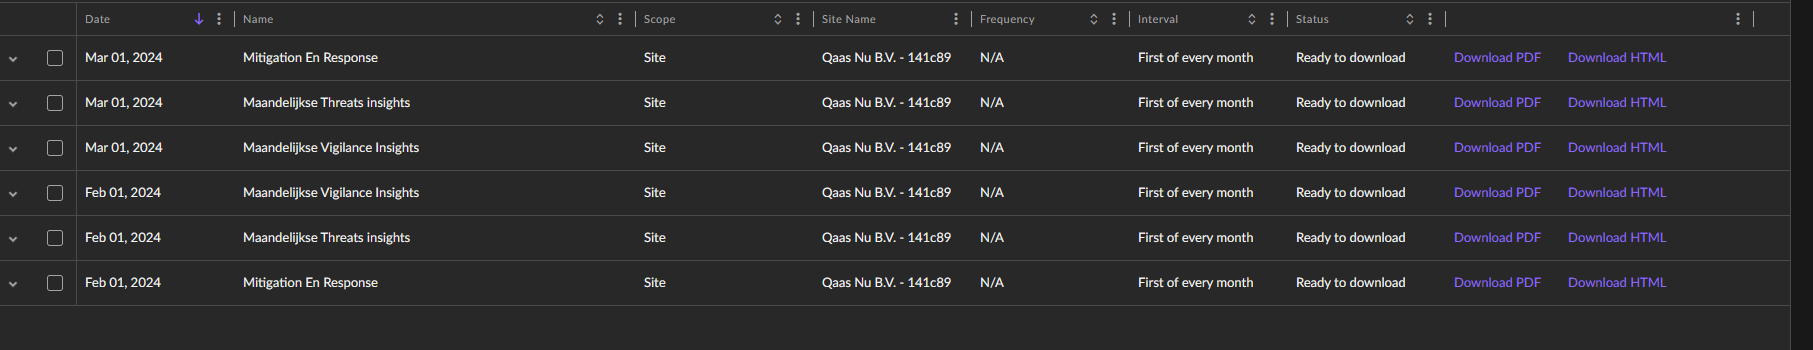
\includegraphics[width=1.0\textwidth]{Figures/SentinelOne/Reports.png}
      \caption{Examples of automatic reports that can be downloaded in SentinelOne}
      \label{fig:Reports}
\end{figure}

\begin{multicols}{2}
      \textbf{Vigilance}

      It is a \acrshort{mdr} service - providing threat monitoring, hunting, and response, to its existing customers. It
      provides a 24/7 \acrshort{soc} with expert analysts and researchers to give customers near real-time threat monitoring,
      in-console threat annotations, and response to threats and suspicious events. Vigilance itself is a separate package from
      SentinelOne.

      The company wishes

      \textbf{\textit{How does SentinelOne get all this information from a device without having them even connected to the Internet?}}

      On a network, before a machine is connected and talks to other devices
      and gateways, it is going to do a broadcast and gives up information about itself. This is called an \acrshort{arp} Request.
      As everything that is talking on Layer 2 is giving out their \acrshort{mac} address for exchange,

      A lot of the times, most switches and routers do not change their default credentials

      As was said before, every single item that is connected to a network is constantly broadcasting information out to the rest of
      network, in order to get and maintain an \acrshort{ip} address to keep accessing the Internet, even when it is not actively using
      it (\textit{see \acrshort{dhcp} Protocol \cite{dhcpProcess}}). In case of an endpoint that has SentinelOne installed on it that
      has Ranger, that Ranger is going to listen to that \acrshort{nic} on that device, then capture and interpret all the data that
      is flowing across the network, called \acrshort{mib}s, thus displaying it on the Console.

      \subsection{SentinelOne API \& SDK}
      SentinelOne provides both an \acrshort{api} and an \acrshort{sdk} to allow users to integrate SentinelOne with other
      security tools and systems. The \acrshort{sdk} is called Nexus Embedded \acrshort{ai} (\textit{\cite{nexusSDK}}), which
      enables organizations to scan files and detect malicious content among them.
\end{multicols}

\begin{lstlisting}[language=Python, caption=SentinelOne SDK implementation]
      from SentinelDFI.scanner import *
      s = Scanner(True)
      verdict = s.scanFile("/home/test_me/malicious.docx")
\end{lstlisting}

\begin{lstlisting}[language=bash]
      File hash: 421ac4189Seed605824fc4cae3e60219febfef
      Verdict: malware
      Score: 0.297529
      Indicators: `Detected VBA Structure,Encrypted file,Encrypted Word Document,Has DDE`
\end{lstlisting}

\begin{multicols}{2}
      Besides \acrshort{sdk}, SentinelOne also provides a \acrshort{rest}ful \acrshort{api} with its comprehensive documentation
      that allows users to interact with the SentinelOne platform programmatically. The \acrshort{api} provides a wide range of
      functionalities, including the ability to retrieve information about devices, incidents, and threats, as well as the ability
      to perform actions such as quarantining devices, remediating threats, and generating reports. The \acrshort{api} is designed
      to work with the Agents, Sentinels, Ranger, and other components of the SentinelOne platform.

      There are many techniques that can be used to create a link (often called an interface). The technology for linking to
      SentinelOne depends on the \textbf{purpose} and \textbf{capabilities} of the software to be linked:
      \begin{itemize}
            \item \textbf{REST, SOAP API/ Webservice}: modern software has its own inputs and outputs to exchange information.
                  This is a sustainble and solid solution for the processing of data
            \item \textbf{CSV/XLSX and XML via (S)FTP}:
            \item \textbf{Webhooks}: like web services, but event based. A signal is automatically sent for each mutation,
                  so that action to process the signal within the software can be taken.
      \end{itemize}

      \textbf{API Token}

      To be able to access SentinelOne APIs, the user needs to have an \acrshort{api} token to prove their identity and that their
      organization has SentinelOne subscription, therefore has right to access data. \acrshort{api} tokens can be created in the
      SentinelOne \acrshort{mgmt} Console.

      The \acrshort{api} token will be shown only once; therefore the user needs to store it in a secure place. The token
      generated by the user is time-limited. To renew the token, the user must generate a new one with the same above-steps.

      \textbf{API Token Storage}
\end{multicols}

\begin{figure}[htbp]
      \centering
      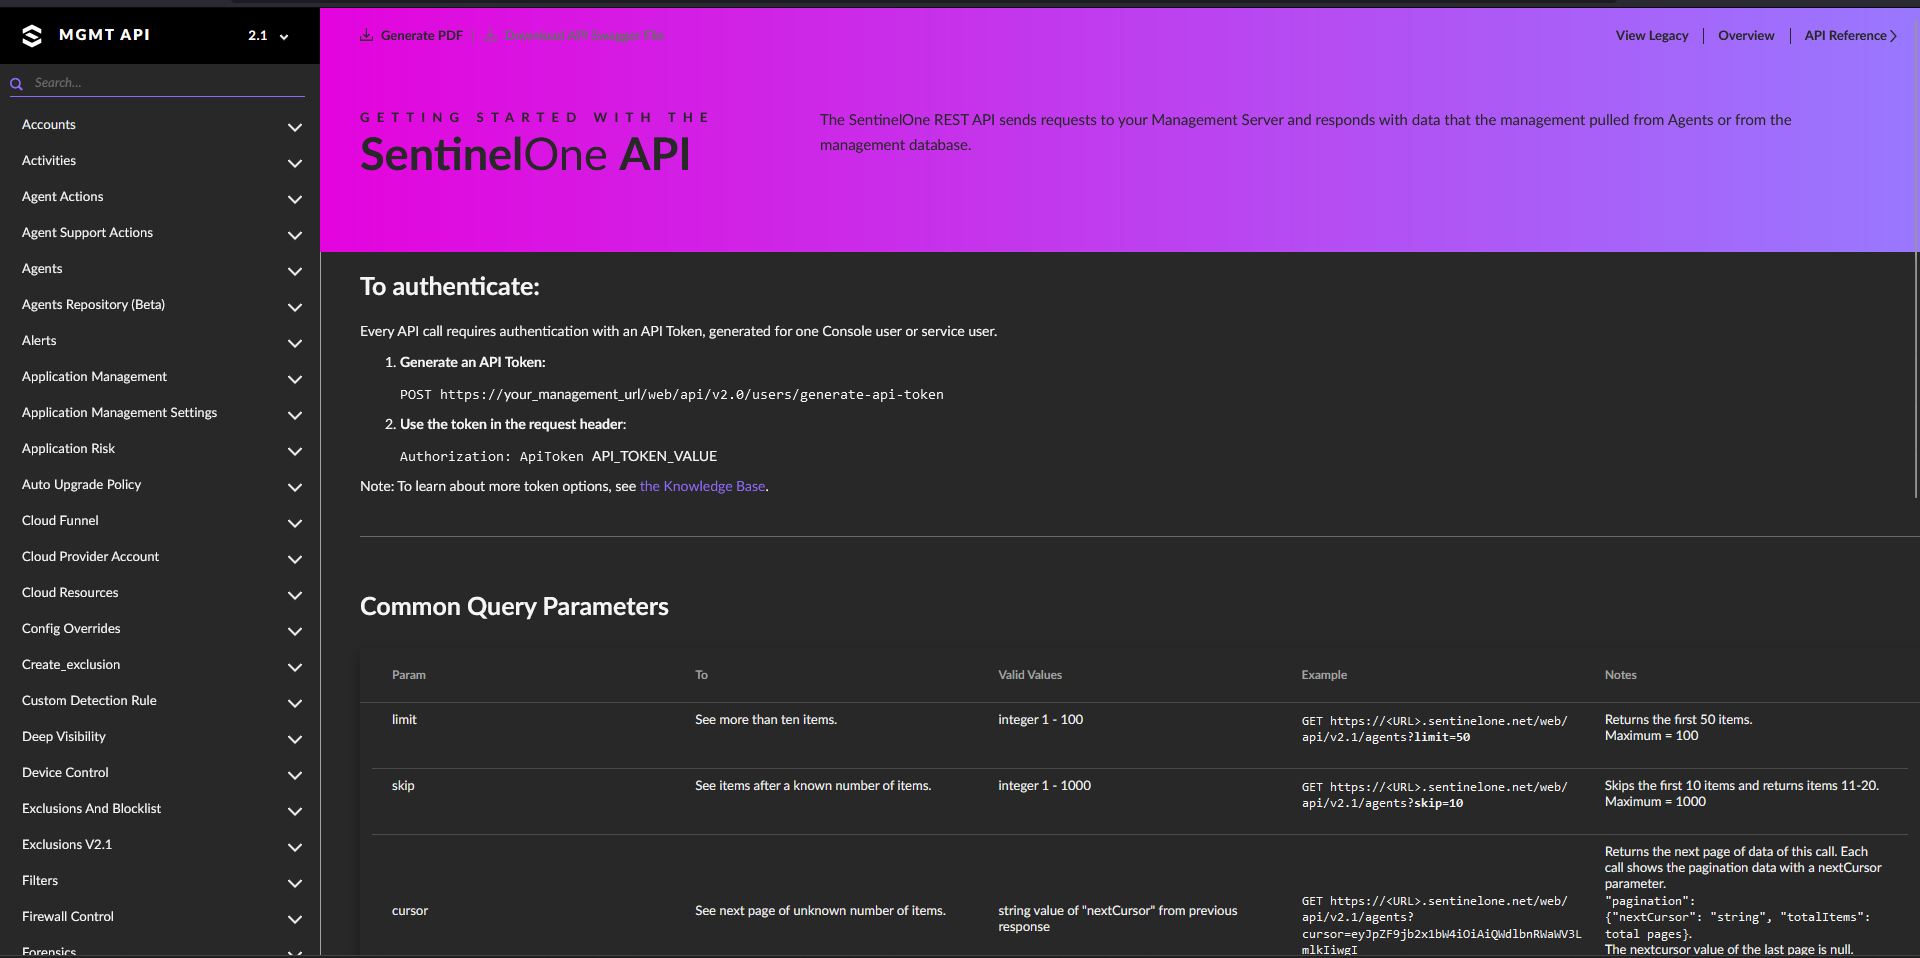
\includegraphics[width=0.8\textwidth]{Figures/SentinelOne/API Doc.png}
      \caption{SentinelOne API Documentation}
\end{figure}

\begin{multicols}{2}
      \section{Research Sub-Question \#3}
      Data visualization is the process of representing complex data (in the form of text and numbers) into a graphical representation,
      such as: interactive charts, dashboards, pie charts, and so on. In the context of this project, the displays should be able to tell
      interesting stories and share findings with diverse audience (the client, helpdesk, and cybersecurity analysts).

      \subsection{Data Visualization Widgets in Flutter}
      In Flutter, there are 2 famous library that supports a wide range of chart types, \href{https://pub.dev/packages/fl_chart}{fl\_chart}
      and \href{https://pub.dev/packages/syncfusion_flutter_charts}{syncfusion\_flutter\_charts}. Each chart type is suitable for a
      specific kind of data and provides a different way to visualize the data. Types of charts in both libraries include 30+ plotting series:
      \begin{itemize}
            \item Line chart: is used to display data points connected by straight line segments. They are commonly used to show trends
                  over time.
            \item Bar chart: it uses rectangular bars to represent data. The length of each bar corresponds to the value it represents.
                  Bar charts are useful for comparing quantities of different categories.
            \item Pie chart: represents data in the form of slices of a pie. Each slice corresponds to a category of the data, and the
                  size of the slice is proportional to the quantity it represents.
            \item Scatter chart: uses dots to represent data points on a two-dimensional plane. They are useful for showing the
                  relationship between two variables.
            \item Radar chart: \acrshort{aka} spider chart or star chart, is a way of comparing multiple quantitative variables. This
                  makes them useful for seeing which variables have similar values or if there are any outliers among each variable.
      \end{itemize}
\end{multicols}

\begin{figure}[htbp]
      \centering
      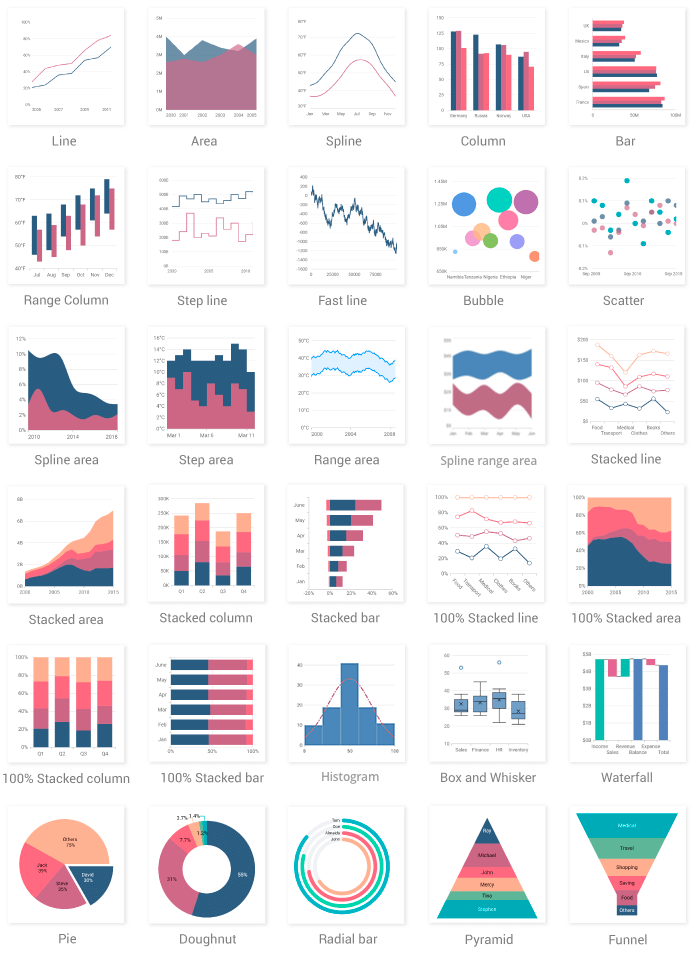
\includegraphics[width=0.8\textwidth]{Figures/Charts.png}
      \caption{Chart types in Flutter fl\_chart}
      \label{fig:charts}
\end{figure}

\begin{multicols}{2}
      Each chart type is easily configured with built-in support for creating stunning visual effects, and any number of series can
      be added to the chart. Features such as markers, data labels, data label builder, animation, gradient fill, dashes, sorting,
      and annotations are easy to incorporate and customize.

      Several main components of each chart type are:
      \begin{itemize}
            \item Chart data: the most important part is the data wanted to be displayed. This could be a simple list of numbers, or
                  more complex data structure, depending on the type of chart.
            \item Chart type: the second most important part is to specify the type of chart.
            \item Axes: the x and y-axes of the chart. The axes provide a reference frame for the data points and can be customized
                  to suit user's needs.
            \item Grid: the grid lines on the chart. These lines can help users better understand the data by providing a reference
                  frame.
            \item Touch response: the way the chart responds to user's touch events. It can be customized by providing different types
                  of interactivity, such as highlighting a data point when it is touched.
      \end{itemize}

      \textbf{Axis Types}

      Axis features such as label intersecting, edge label placement, label rotation, axis opposition, inverse axis, and multiple axis
      allow users to customize axis elements to make an axis more readable. Four of the axis types that are supported are:
      \begin{itemize}
            \item Numeric
            \item Category
            \item Date-time
            \item Logarithmic
      \end{itemize}

      \textbf{User Interaction}

      The package greatly enhance \acrshort{ux} by adding the following functionalities:
      \begin{itemize}
            \item Zooming and panning
            \item Crosshairs
            \item Trackballs
            \item Drilling down
            \item Events
            \item Selection
            \item Tooltips
      \end{itemize}

      \textbf{Legend}

      The package also supports legends, which display additional information about a chart series. The legends can be used to
      collapse the series and can be wrapped or scrolled if items exceed the available bounds.

      \subsection{Comparison to other EDR solutions}
      To determine the best visualization techniques for SentinelOne, a comparison to other \acrshort{edr} solutions is needed.
      In this section, the author has looked into other alternatives to SentinelOne, which are a single \acrshort{epp}/\acrshort{edr}
      solution, created as a complete replacement of legacy \acrshort{av}. Please keep in mind that in this sub-question, only the
      visualization techniques will be assessed, compared, contrasted, evaluated, and discussed. The other factors such as pricing,
      technologies, and features will not be discussed in this sub-question.

      \subsubsection{Heimdal\textregistered}

      On the homepage, information about each of the products/modules that are active under the current customer account is shown. The
      chart, which can be seen include a variety of Bar charts, Pie charts, and Line charts, include data regarding attacks,
      vulnerabilities, detections, infected/quarantined files, blocked/allowed processes, third-party application vulnerabilities or
      \acrshort{os} updates, and quarantined/rejected e-mails.

      \subsubsection{CrowdStrike}


      \subsubsection{Trend Micro} % Fukujima
      Trend Micro Apex One has customizable contents and layout of their dashboard. Workload Security uses Session to save user's
      settings and remember the last view of the dashboard the next time the user log in.
      The colour here is a bit basic with only the typical
      red, green, blue, and yellow.

      Based on the three examples above, some conclusion can be drawn about the techniques they use in their dashboard:

      \textbf{Visualization techniques}

      All three solutions use a combination and types of bar charts, pie charts, and line charts to display data. This due to the fact
      that the type of data they are trying to display is categorical and numerical data. Categorical data is data that can be divided
      into distinct groups or categories with no inherent order, and one category  can only have one value.

      Pie charts are used to visualize relative proportions or percentages of different categories within a dataset. Each category is
      represented by a slice of pie, with the size of each slice corresponding to the proportion of that category relative to the
      whole dataset.

      Bar graphs are used to compare the quantities or frequencies of different categories. Each category is represented by a separate
      bar, with the height (or length, in horizontal bar graphs) of the bar indicating the value of that category.

      In the case of SentinelOne integration to the \acrshort{qaas} app, both bar and pie charts can be used with the addition of
      line charts to display the timeline of a Threat Incident, and Scatter charts to show the relationship between two variables.

      \textbf{Customizable Widgets}

      All three solutions allow users to customize the layout and contents of their dashboards. This is important as different users
      may have different preferences and requirements for the data they want to see. Customizable widgets allow users to choose which
      data they want to display, how they want to display it, and where they want to display it on the dashboard.

      The SentinelOne dashboard of the \acrshort{qaas} app should have this functionality, therefore it should store user's preference
      \textbf{Coloring}
      % \subsection{Huntress}
      % CrowdStrike Falcon
      % \subsection{Datto RMM}
      % \subsection{Sophos}
      % \subsection{Carbon Black}
      % \subsection{Kaspersky Endpoint Security}
      % \subsection{Bitdefender}
      % Bitdefender Gravity Zone
      % \subsection{McAfee}
      % \subsection{Symantec}
      % \subsection{Trend Micro}
      % \subsection{Cynet 369}
      % \subsection{Microsoft Defender for Endpoint}
      % \section{Research Sub-Question \#4}
\end{multicols}